% =====================================================================
%  Inline Edge Identifiers for Multi-Edge Property Graphs
%  arXiv-style preprint. Self-contained: no external .bib required.
%  Build:  pdflatex tensor && pdflatex tensor
% =====================================================================
\documentclass[11pt,a4paper]{article}

\usepackage[T1]{fontenc}
\usepackage[utf8]{inputenc}
\usepackage[margin=1in]{geometry}
\usepackage{amsmath}
\usepackage{amssymb}
\usepackage{amsthm}
\usepackage{booktabs}
\usepackage{xcolor}
\usepackage{listings}
\usepackage{algorithm}
\usepackage{algpseudocode}
\usepackage{tikz}
\usetikzlibrary{positioning,arrows.meta,fit,backgrounds}
\usepackage[hidelinks]{hyperref}

\theoremstyle{plain}
\newtheorem{theorem}{Theorem}
\newtheorem{lemma}[theorem]{Lemma}
\newtheorem{proposition}[theorem]{Proposition}
\theoremstyle{definition}
\newtheorem{definition}[theorem]{Definition}
\newtheorem{invariant}{Invariant}
\theoremstyle{remark}
\newtheorem{remark}[theorem]{Remark}

\newcommand{\M}{\mathsf{M}}
\newcommand{\dom}{\operatorname{dom}}

% switch/case for algpseudocode (not provided by default)
\algnewcommand\algorithmicswitch{\textbf{switch}}
\algnewcommand\algorithmiccase{\textbf{case}}
\algdef{SE}[SWITCH]{Switch}{EndSwitch}[1]
  {\algorithmicswitch\ #1\ \algorithmicdo}{\algorithmicend\ \algorithmicswitch}
\algdef{SE}[CASE]{Case}{EndCase}[1]
  {\algorithmiccase\ #1}{\algorithmicend\ \algorithmiccase}

% float placement: the default \topfraction starves the wider tables, which
% then queue behind one another and land pages away from their discussion.
\renewcommand{\topfraction}{0.85}
\renewcommand{\bottomfraction}{0.7}
\renewcommand{\textfraction}{0.12}
\renewcommand{\floatpagefraction}{0.7}

\definecolor{kw}{RGB}{0,90,160}
\definecolor{cmt}{RGB}{100,110,100}
\definecolor{str}{RGB}{150,60,20}
\lstdefinestyle{rust}{
  basicstyle=\ttfamily\footnotesize,
  keywordstyle=\color{kw}\bfseries,
  commentstyle=\color{cmt}\itshape,
  stringstyle=\color{str},
  showstringspaces=false,
  columns=fullflexible,
  breaklines=true,
  frame=single,
  framesep=4pt,
  rulecolor=\color{black!25},
  morekeywords={fn,let,mut,match,if,else,for,in,pub,struct,enum,impl,Self,self,
    return,continue,break,Some,None,u64,bool,usize,const,use,where,as,true,false},
  morecomment=[l]{//},
}
\lstset{style=rust}

% ---------------------------------------------------------------------
\title{\textbf{Inline Edge Identifiers for Multi-Edge Property Graphs:\\
A Sentinel-Promotion Tensor over Sparse Linear Algebra}}

\author{%
Guy Korland\thanks{\texttt{guy.korland@falkordb.com}} \and
Roi Lipman\thanks{\texttt{roi.lipman@falkordb.com}} \and
Dvir Dukhan\thanks{\texttt{dvir.dukhan@falkordb.com}} \and
Avi Avni\thanks{\texttt{avi.avni@falkordb.com}}
\\[0.6em]
FalkorDB\\
\small\texttt{https://github.com/FalkorDB/FalkorDB}}

\date{\today}

\begin{document}
\maketitle

\begin{abstract}
Graph databases built on sparse linear algebra represent a graph as a set of
adjacency matrices and express traversal as matrix--matrix and
matrix--vector products. The representation is elegant but structurally
lossy for \emph{property multigraphs}: a matrix cell holds one value, whereas
a property graph may connect an ordered node pair by arbitrarily many
distinct edges, each carrying its own identity and property map. The
canonical remedy is to store a container per cell --- conceptually a
three-dimensional tensor $T[i,j,\cdot]$ --- which restores expressiveness
but pays a per-cell container in the overwhelmingly common case of exactly
one edge per pair.

We describe and analyse the design of \texttt{Tensor}, the per-relationship-type
edge store of FalkorDB's Rust storage engine. Its central idea is
\emph{inline-first representation with sentinel promotion}: the forward
adjacency matrix is \texttt{UINT64}-valued and stores a single edge's
identifier \emph{directly} as the matrix value, so a simple graph requires no
auxiliary edge structure whatsoever. A reserved sentinel value $\M = 2^{64}-1$
in the cell announces that the pair has become multi-edge, at which point
\emph{all} of the pair's identifiers migrate to a single global hypersparse
overflow matrix keyed by a packed $(\text{src},\text{dst})$ compound key.
The scheme is provably safe --- edge identifiers are bounded by the GraphBLAS
index limit $2^{60}-1$ and therefore cannot collide with the sentinel --- and
it reduces the steady-state cost of a single-edge pair to one $\langle$32-bit
index, 64-bit value$\rangle$ pair, roughly $12$ bytes, with no per-pair
container object and no second matrix.

The structure is simultaneously a multi-version concurrency control (MVCC)
object: three delta layers (committed base, pending additions, pending
deletion mask) give snapshot isolation over the same cells. We show that
value-carrying cells force a strictly richer delta algebra than the
Boolean case --- a pending layer must be able to \emph{shadow} a live
committed value rather than only add to or subtract from a pattern --- and we
give the resulting ten-state per-pair automaton, a closed-form cardinality
identity, and a proof that the three-way sorted-merge iterator streams
exactly the effective edge multiset in $(\text{src},\text{dst},\text{id})$
order. The invariant set, the automaton and both theorems are machine-checked in
Lean 4 against a model transcribed from the Rust --- $7{,}071$ lines and $460$
theorems, with no \texttt{sorry} and no bespoke axiom --- which found two
unreachable branches in the shipped code, one of which would have fabricated a
valid edge identifier had the invariant it rested on ever broken. We are
explicit about what such a proof does not establish, since it binds a model and
not the binary. We further state two rules that embedding such a
structure in a non-blocking sparse-linear-algebra runtime imposes: keep
operators pattern-only on identifier-carrying matrices, because a
value-carrying operator typecasts the identifier $0$ into an entry that valued
masks treat as absent; and discharge any ``this object is materialised''
invariant by enumerating the calls that can queue work on it, including
capacity changes that read as metadata. Both are cheap to follow, expensive to
retrofit, and pinned by regression tests. We close with an
analytic cost model and an empirical evaluation against the pointer-tagged
container-per-cell design used by FalkorDB's C implementation, measured both as
whole queries and at the data-structure boundary on both sides. Inline-first
costs a quarter as much to promote a pair and a quarter as many bytes per edge
once a pair holds two edges; its per-edge iteration is slightly \emph{worse}, so the
engine-level scan advantage belongs to the engine and not to edge storage. Two
of our own engine-level attributions turn out to overstate storage cost by
$1.6\times$ and $5.1\times$, which is the sharpest argument we can offer for
measuring at the boundary. The design's distinguishing promotion/demotion
transition, predicted to be a small constant, was a quadratic in our
implementation; we give the diagnosis, the fix, and the residual constant factor
of about three that remains. We close with the domain restrictions the compound
key imposes.
\end{abstract}

\noindent\textbf{Keywords:} property graphs, multigraphs, GraphBLAS, sparse
matrices, hypersparse, multi-version concurrency control, delta encoding,
graph databases

% =====================================================================
\section{Introduction}
\label{sec:intro}

The linear-algebraic view of graph computation --- represent a graph by its
adjacency matrix, express traversal as products over a semiring --- is old
\cite{kepnergilbert2011} and, since the GraphBLAS standardisation effort
\cite{mattson2013,kepner2016,brock2021spec} and the arrival of a
high-performance reference implementation in SuiteSparse:GraphBLAS
\cite{davis2019toms,davis2023toms}, practical. Several systems now use it as
their storage substrate rather than merely as an algorithm library; FalkorDB
(originally RedisGraph \cite{cailliau2019}) executes openCypher
\cite{francis2018cypher} query plans directly against GraphBLAS matrices,
turning a pattern match into a chain of masked matrix products.

The mismatch this paper addresses is narrow and concrete. A matrix is a
partial function $A : \mathbb{N} \times \mathbb{N} \rightharpoonup S$: an
ordered pair maps to \emph{at most one} value. A property graph
\cite{angles2017foundations} is a multigraph: an ordered node pair may be
connected by many edges of the same type, each a first-class entity with its
own identifier and property map. ``Alice \texttt{TRANSFERRED} Bob'' is not a
fact about a pair of accounts, it is a set of facts, each with its own amount
and timestamp, each of which a query may bind, filter, project and delete
individually. The adjacency matrix can record that the pair is connected; it
cannot, by itself, record \emph{which} edges connect it.

The textbook fix is to lift the value domain from a scalar to a container,
giving a three-dimensional structure $T$ where $T[i,j,\cdot]$ enumerates the
identifiers joining $i$ to $j$. FalkorDB's C implementation does exactly
this, storing a tagged \texttt{GrB\_Vector} handle in the cell: the
most-significant bit of the 64-bit value distinguishes ``this is a scalar
edge id'' from ``this is a pointer to a vector of edge ids.''\footnote{See
\texttt{src/graph/tensor/tensor.h} in the FalkorDB C sources: the macros
\texttt{SCALAR\_ENTRY(x)} and \texttt{AS\_VECTOR(x)} implement precisely this
pointer tagging.} This is expressive and, for genuinely multi-edge graphs,
efficient. It is also unsatisfying for the case that dominates real
workloads, where almost every connected pair has exactly one edge: the
representation is fully general and pays for generality everywhere.

\paragraph{Contributions.}
This paper documents and analyses the design that replaces it in FalkorDB's
Rust storage engine. Specifically:

\begin{enumerate}
  \item \textbf{Inline-first representation with sentinel promotion}
        (\S\ref{sec:representation}). The forward adjacency matrix is
        \texttt{UINT64} rather than \texttt{BOOL} and stores a lone edge's
        identifier \emph{as} the cell value. A reserved sentinel
        $\M = 2^{64}-1$ marks a pair that has outgrown one edge; only then do
        identifiers move to an auxiliary structure, and \emph{all} of them
        move, so the cell value is never ambiguous. We prove the sentinel
        cannot collide with a real identifier
        (Lemma~\ref{lem:sentinel}).
  \item \textbf{A single global overflow matrix instead of per-cell
        containers} (\S\ref{sec:compound}). Multi-edge identifiers live in one
        hypersparse \cite{bulucgilbert2008} Boolean matrix indexed by a
        \emph{compound key} $\kappa(s,d) = (s \ll 32) \mathbin{|} d$ in the
        row dimension and by edge identifier in the column dimension. This
        removes $N$ container objects and their allocation, lifetime and
        serialisation obligations in exchange for one wide, mostly empty
        matrix that GraphBLAS already stores in $O(\mathrm{nvals})$ space.
  \item \textbf{A delta algebra for value-carrying MVCC layers}
        (\S\ref{sec:deltas}). Boolean delta matrices need only
        \emph{add} to and \emph{subtract} from a pattern. Value-carrying
        layers additionally need in-place \emph{update}, which we implement by
        allowing the pending layer to \emph{shadow} a live committed cell
        without masking it. We give the invariants this requires, the induced
        ten-state per-pair automaton
        (\S\ref{sec:automaton}, Figure~\ref{fig:automaton}), and a
        \emph{cancel-to-clean} normalisation rule that keeps the state space
        finite and the cardinality identity exact.
  \item \textbf{A closed-form edge count and a streaming-iteration theorem}
        (\S\ref{sec:correctness}). We prove
        $|E| = |m| + |dp| - |dm| - |dp \cap m| - \textit{multi} + |me|$
        (Theorem~\ref{thm:count}) --- computable from GraphBLAS metadata plus a
        single structural intersection, with no scan --- and that the
        three-way sorted merge emits each effective edge exactly once in
        lexicographic order without materialising an intermediate matrix
        (Theorem~\ref{thm:iter}).
  \item \textbf{A machine-checked development, and an account of its limits}
        (\S\ref{sec:mechanised}). $7{,}071$ lines and $460$ theorems of Lean 4
        over a model transcribed operation by operation from the Rust, in two
        layers so that the tensor's use of its Boolean sub-structure is proved
        rather than assumed. It pays for itself by finding two unreachable
        branches in the shipped code --- and it binds a model, not a binary, so
        we say where the correspondence rests and where the code has since moved
        ahead of it.
  \item \textbf{Two rules the host runtime imposes}
        (\S\ref{sec:hazards}). \emph{Keep operators pattern-only on
        identifier-carrying matrices}: a value-propagating operator typecasts
        the \texttt{UINT64} identifier $0$ into a stored \texttt{false},
        which valued masks treat as absent, so the densest-allocated
        identifier in the graph is the one silently lost. \emph{Discharge
        materialisation invariants by enumerating callers}: authorship is not
        the same as queued work, and a capacity change that reads as metadata
        can leave the committed base pending. We give the operator choices and
        the call-site discipline that satisfy both.
  \item \textbf{An analytic cost and space model} (\S\ref{sec:cost})
        \textbf{an empirical evaluation against the container-per-cell
        implementation at two grains} (\S\ref{sec:eval}). A multiplicity sweep
        of whole queries at fixed $|E|$, and both structures measured as
        structures --- a C harness linked against the shipped archive with no
        stubs, and Rust measurement tests. Promotion and multi-edge space come
        out as the design predicts ($0.24\times$ and $0.25\times$); iteration
        does not, being slightly worse per edge, so the engine-level scan
        advantage is not edge storage; and two of our own engine-level
        attributions overstate storage cost by $1.6\times$ and $5.1\times$. The
        promotion/demotion transition, predicted to be a small constant, was a
        quadratic in our implementation: we give the measurement, the
        instrumented cause, the fix, and the $3\times$ residual.
  \item \textbf{An explicit account of the design's \emph{domain
        restrictions}} (\S\ref{sec:limits}), including the
        observation that although the compound-key guard admits node
        identifiers up to $2^{32}-1$, the overflow matrix's dimension bounds
        the source identifier of a multi-edge pair by $2^{28}$.
\end{enumerate}

\paragraph{Scope.} This is a design and analysis paper about a single data
structure, written against a specific artifact: \texttt{Tensor} in
\texttt{graph/src/graph/graphblas/tensor.rs} in the FalkorDB repository, as
given under Availability. Our cost model (\S\ref{sec:cost}) is
analytic --- space and operation costs derived from the storage formats and the
GraphBLAS operations invoked --- and \S\ref{sec:eval} measures it, because the
design's central claim, that inline-first is cheaper for the common case, is a
claim about constants and constants deserve measurement. That evaluation has two grains: a
multiplicity sweep of whole queries against design (A) as shipped in FalkorDB's
C implementation, and both structures measured as structures, with a C harness
linked against the shipped archive. The second grain corrects the first in
places, which we report as a finding rather than as errata. It confirms the
space and promotion claims, shows the scan advantage is not edge storage, and
refutes the paper's own prediction about the promotion/demotion transition,
which was a quadratic in our implementation until the fix of
\S\ref{sec:evalosc} made it a constant still about $3\times$ (A)'s. Design (B)
remains unimplemented, so every (B) figure here is a bound or a model, and
\S\ref{sec:limits} is precise about what that leaves unmeasured. The fold policy of \S\ref{sec:folding} rested on measured constants
already, for the separate reason that the rule they determine is sensitive to
them.

The invariants, the per-pair automaton and the theorems of
\S\ref{sec:correctness} are machine-checked in Lean 4 against a model
transcribed from the Rust (\S\ref{sec:mechanised}). That is a claim about the
model's correspondence to the code, which no proof can establish; we say what
that correspondence rests on and where it stops.

% =====================================================================
\section{Background}
\label{sec:background}

\subsection{GraphBLAS, sparsity formats, and non-blocking execution}

GraphBLAS \cite{brock2021spec} specifies opaque sparse matrix and vector
objects over user-selectable semirings, with masked, accumulated operations
as the primitive vocabulary. Three properties of the SuiteSparse
implementation \cite{davis2019toms,davis2023toms} shape our design.

\paragraph{Multiple storage formats, including hypersparse.}
SuiteSparse selects among \emph{full}, \emph{bitmap}, \emph{sparse}
(compressed, CSR/CSC-like \cite{gustavson1978}) and \emph{hypersparse}
representations. The hypersparse format \cite{bulucgilbert2008} additionally
compresses the vector dimension, storing only the indices of non-empty
vectors, so a matrix's space is $O(\mathrm{nvals})$ \emph{independent of its
declared dimensions}. This is what makes a $(2^{60}-1) \times (2^{60}-1)$
matrix a sensible object to allocate. The artifact leans on it deliberately:
matrices are pinned to \texttt{SPARSE | HYPERSPARSE} so that the runtime never
promotes a mostly-empty matrix to bitmap (which would make every subsequent
fold pay a whole-bitmap \texttt{memset}), and delta layers are pinned
\emph{fully} hypersparse --- a small delta over a matrix whose row capacity
has been inflated to a million by a bulk load costs $O(\mathrm{nvec})$ rather
than $O(\mathrm{nrows})$ per materialisation.

\paragraph{Non-blocking execution.}
Operations may be queued rather than performed. A matrix carries
\emph{pending tuples} and \emph{zombies} until a \texttt{GrB\_Matrix\_wait}
materialises it. This is a performance feature --- $n$ scattered
\texttt{setElement} calls become one bulk build --- but it leaks into the
design of anything built on top, because a \emph{read} of a pending matrix
must first materialise it. A data structure that interleaves reads and writes
element-wise therefore risks $\Theta(n)$ materialisations for $n$ writes; we
return to this in \S\ref{sec:insert}.

\paragraph{Typed operators.}
Every operation names an operator or semiring, and the choice determines
whether operand \emph{values} are read. \texttt{GxB\_ANY\_PAIR\_BOOL} and
\texttt{GxB\_ONE\_BOOL} inspect only the sparsity pattern;
\texttt{GrB\_eWiseAdd} with a binary operator propagates and \emph{typecasts}
values from cells present on only one side. When the value domain is edge
identifiers, this distinction is a correctness boundary
(\S\ref{sec:hazard-zero}).

\subsection{Matrices as the storage layer of a property graph}

FalkorDB assigns each node a dense integer identifier and each relationship
type its own $n \times n$ matrix; a label becomes a diagonal matrix, and a
Cypher pattern becomes a masked product chain. Node identifiers index rows
and columns; the value domain of a relationship matrix is what this paper is
about.

\subsection{Delta matrices and snapshot isolation}
\label{sec:bg-delta}

To let readers proceed against a consistent snapshot while a writer mutates
\cite{bernstein1983mvcc,neumann2015mvcc}, each logical matrix is a triple of
physical matrices, in the artifact's naming: a committed base $m$, a
\emph{delta-plus} $dp$ of pending additions, and a \emph{delta-minus} $dm$ of
pending deletions. The effective content is
\[
  \mathcal{E} \;=\; (m \setminus dm) \cup dp ,
\]
and once a delta is large enough to earn the rewrite it is folded into the base
and cleared --- structurally the same amortisation as an LSM tree's compaction
\cite{oneil1996lsm}, at one level, though \S\ref{sec:folding} shows the sizing
rule differs from an LSM ratio for a reason specific to this setting. Each
physical matrix sits behind
a copy-on-write cell, so opening a write transaction clones handles in $O(1)$
and the first mutation of a given matrix pays its deep copy; read-only
transactions pay nothing.

For \emph{Boolean} layers this is complete, and the invariants are the strict
ones: $dm \subseteq \dom(m)$ and $\dom(dp) \cap \dom(m) = \emptyset$. A cell
is present or absent, so ``update'' is not an operation. Once cells carry
values, it is, and \S\ref{sec:deltas} shows that the natural encoding of an
update breaks the second invariant on purpose.

% =====================================================================
\section{Design space}
\label{sec:designspace}

Fix a relationship type $r$ and let $P$ be its set of connected ordered node
pairs, $E$ its edge set, and $\mu = |E|/|P|$ the mean multiplicity. Three
designs answer ``where do the identifiers live?''

\paragraph{(A) Container per cell (pointer tagging).}
The cell holds either a scalar identifier or a tagged pointer to a container
of identifiers, discriminated by a reserved bit. This is FalkorDB's C design.
Reads are direct; the cost is one heap-allocated container object per
multi-edge pair, plus the obligations that come with storing raw pointers
inside matrix values: the containers are invisible to the matrix's own
lifetime management, so duplication, serialisation, and deallocation must all
walk the cells and handle the tagged case explicitly, and any bulk GraphBLAS
operation that would \emph{copy} values is unsafe unless every consumer knows
the tagging discipline.

\paragraph{(B) Always-materialised auxiliary matrix.}
Keep the adjacency matrix Boolean and hold every identifier in a second
$|P| \times |E|$-shaped structure. Uniform and pointer-free, but a simple
graph --- $\mu = 1$, the common case --- pays a second matrix, a second index
per edge, and a second traversal per lookup for information the adjacency
matrix could have carried itself.

\paragraph{(C) Inline-first with lazy overflow (this work).}
Make the adjacency matrix \texttt{UINT64} and store a lone identifier in the
cell. Allocate the auxiliary matrix but leave it empty until some pair gains a
second edge; then \emph{promote} that pair, moving all its identifiers to the
auxiliary matrix and writing the sentinel $\M$ into the cell. On removal,
\emph{demote} symmetrically. A graph with $\mu = 1$ never touches the
auxiliary matrix and never allocates a container; a graph with large $\mu$
degenerates gracefully to (B) plus one wasted cell per pair.

\begin{table}[t]
\centering
\small
\begin{tabular}{@{}lccc@{}}
\toprule
 & \textbf{(A) container/cell} & \textbf{(B) always aux.} & \textbf{(C) inline-first} \\
\midrule
Space, single-edge pair      & 1 cell                & 1 cell $+$ 1 aux.\ entry & 1 cell \\
Space, $k$-edge pair ($k\ge2$) & 1 cell $+$ container($k$) & 1 cell $+$ $k$ aux.    & 1 cell $+$ $k$ aux. \\
Aux.\ structure when $\mu=1$ & absent                & fully materialised       & allocated, empty \\
Heap objects outside GraphBLAS & $|\{k\ge2\}|$        & none                     & none \\
Point read, single edge      & 1 lookup              & 2 lookups                & 1 lookup \\
Point read, $k$-edge         & 1 lookup $+$ scan     & 2 lookups $+$ scan       & 1 lookup $+$ row scan \\
Values safe under bulk ops   & no (tagged pointers)  & yes                      & yes (sentinel) \\
Transition cost on 2nd edge  & allocate container    & none                     & promote: 2 aux.\ writes \\
\bottomrule
\end{tabular}
\caption{The three designs. (C) is (B) with the $\mu = 1$ case specialised
into the adjacency matrix, and (A) with the heap containers replaced by rows
of one global matrix. Its distinguishing cost is the promotion/demotion
transition, which (A) and (B) do not have.}
\label{tab:designspace}
\end{table}

Table~\ref{tab:designspace} summarises. Design (C) buys the common case at
the price of a state transition and the invariant discipline that transition
requires; the rest of this paper is largely about that price, and
\S\ref{sec:eval} measures it --- and finds its two halves pointing opposite
ways. \emph{Promotion} is where (C) wins most decisively, because it is exactly
where (A) allocates the heap container this table gives it: $0.24\times$ (A)'s
cost, alongside $0.25\times$ its space per multi-edge pair. \emph{Demotion} is
where (C) loses: even after a defect fix it costs about three times what (A)
pays for the same logical change. The transition is the design's distinguishing
cost in both directions, and the design is right about one of them.

% =====================================================================
\section{Representation}
\label{sec:representation}

\subsection{Components}
\label{sec:components}

\begin{lstlisting}
pub struct Tensor {
    m:  Cow<Matrix<u64>>,        // committed forward adjacency: src -> dst = edge id | MULTI
    dp: Delta<u64>,              // pending additions / in-place value updates
    dm: Delta<bool>,             // pending deletions (mask over m)
    mt: VersionedMatrix<bool>,   // backward adjacency: dst -> src, structure only
    me: VersionedMatrix<bool>,   // overflow: compound_key(src,dst) -> edge id
    needs_flush: AtomicBool,     // a latched fold is executable now
}

// One delta layer plus the bookkeeping the fold policy reads about it.
struct Delta<T> {
    layer: Cow<Matrix<T>>,
    count: AtomicU64,            // approximate |layer|, maintained without GraphBLAS calls
    tx_nvals: u64,               // count at version creation: count - tx_nvals is this tx's share
    fold: AtomicBool,            // decision latched here, executed by the next flush
}

pub const MULTI_EDGE: u64 = u64::MAX;
pub const GrB_INDEX_MAX: u64 = (1u64 << 60) - 1;
\end{lstlisting}

Figure~\ref{fig:components} shows how the five matrices relate.

The number of multi-edge pairs, written $\textit{multi}$ throughout and needed
by the cardinality identity of \S\ref{sec:correctness}, is \emph{not} a field.
It is derived from $me$ on demand; \S\ref{sec:limits} gives the derivation and
why an earlier revision of this structure carried it as a maintained counter
instead.

Three asymmetries are deliberate. First, the forward adjacency is \emph{not}
wrapped in the generic \texttt{VersionedMatrix}; the tensor owns its layers
directly, because the delta semantics it needs (\S\ref{sec:deltas}) are
strictly richer than the Boolean ones and the edge-identifier meaning of the
values must stay local to this module. Second, the backward matrix
$mt$ is Boolean: it mirrors the effective forward \emph{structure} and stores
no identifiers at all. Incoming-edge iteration recovers identifiers by
looking the pair up in the forward layers. This trades one point lookup per
backward pair for not duplicating every identifier in the graph --- a
worthwhile trade given that the forward matrix is the authority and any
duplicated copy would be a second thing to keep consistent.

Third, each delta is bundled with its own fold bookkeeping rather than the
owner carrying parallel \texttt{dp\_}/\texttt{dm\_} fields. That is what keeps
the policy of \S\ref{sec:folding} out of the operations: a mutation moves
\texttt{count} alongside the layer write, and nothing else in the tensor
mentions folding. \texttt{count} is deliberately \emph{approximate} --- asking
GraphBLAS for a delta's true size forces its pending tuples to merge, which is
the $O(|\delta|)$ cost the policy exists to bound --- so it is reconciled to the
exact size only when something materialises the layer anyway. Because the same
type is used by the Boolean matrices, the two layers differ only in element
type: \texttt{Delta<u64>} carries identifiers, \texttt{Delta<bool>} a mask.

\begin{figure}[t]
\centering
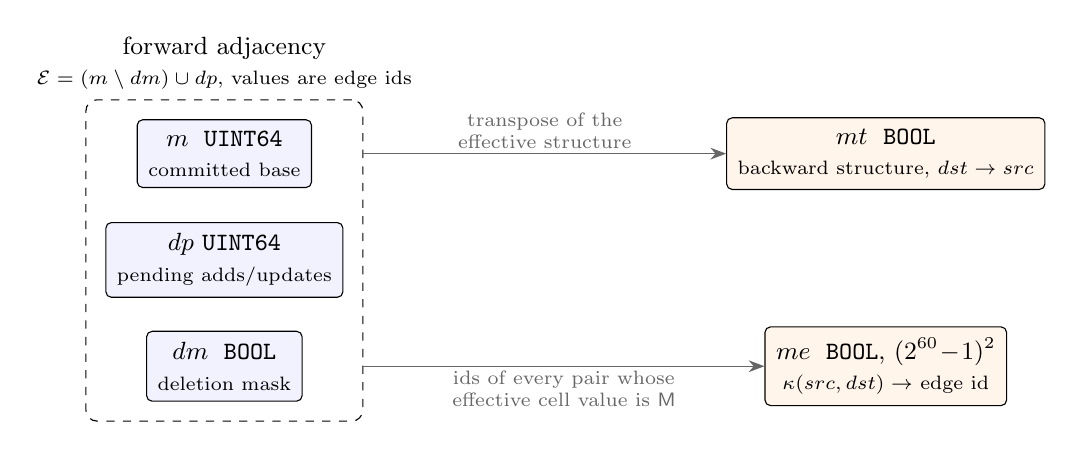
\begin{tikzpicture}[
  font=\small,
  box/.style={draw,rounded corners=2pt,minimum height=8mm,align=center,inner sep=4pt},
  lay/.style={box,fill=blue!5},
  aux/.style={box,fill=orange!8},
  >={Stealth[length=2mm]}
]
\node[lay] (m)  at (0,0)      {$m$ \;\texttt{UINT64}\\\scriptsize committed base};
\node[lay] (dp) at (0,-1.35)  {$dp$ \texttt{UINT64}\\\scriptsize pending adds/updates};
\node[lay] (dm) at (0,-2.7)   {$dm$ \;\texttt{BOOL}\\\scriptsize deletion mask};
\node[draw,dashed,rounded corners,fit=(m)(dp)(dm),inner sep=7pt,
      label={[align=center]above:forward adjacency\\\scriptsize
      $\mathcal{E}=(m\setminus dm)\cup dp$, values are edge ids}] (fwd) {};

\node[aux] (mt) at (8.4,0)     {$mt$ \;\texttt{BOOL}\\\scriptsize backward structure, $dst \to src$};
\node[aux] (me) at (8.4,-2.7)  {$me$ \;\texttt{BOOL}, $(2^{60}\!-\!1)^2$\\\scriptsize $\kappa(src,dst) \to$ edge id};

\draw[->,black!60] (fwd.east |- m) -- node[midway,above,font=\scriptsize,
      align=center,fill=white,inner sep=1.5pt]
      {transpose of the\\effective structure} (mt.west);
\draw[->,black!60] (fwd.east |- dm) -- node[midway,below,font=\scriptsize,
      align=center,fill=white,inner sep=1.5pt]
      {ids of every pair whose\\effective cell value is $\M$} (me.west);
\end{tikzpicture}
\caption{Components. The three forward layers carry edge identifiers as
matrix values; $mt$ and $me$ are Boolean. $me$ is empty unless some pair has
more than one edge, so a simple graph consists of the forward layers and a
Boolean transpose.}
\label{fig:components}
\end{figure}

\subsection{The sentinel and why it is safe}

\begin{lemma}[Sentinel non-collision]
\label{lem:sentinel}
No real edge identifier equals $\M = 2^{64}-1$.
\end{lemma}

\begin{proof}
Edge identifiers are used as \emph{column indices} of the overflow matrix
$me$, whose declared dimensions are $\texttt{GrB\_INDEX\_MAX} = 2^{60}-1$ in
both directions. Any identifier that could ever be stored is therefore
$< 2^{60}-1 < 2^{64}-1$. Identifiers are allocated densely from $0$ upward by
the graph's relationship-identifier allocator, so the bound is not merely
sufficient but a hard ceiling imposed by the storage. Hence the sentinel is
outside the identifier domain.
\end{proof}

This is the reason design (C) is available at all. Note the contrast with
design (A): pointer tagging reserves a \emph{bit}, which constrains the value
domain to $2^{63}$ and makes every value observation conditional on the tag;
sentinel reservation removes a single \emph{point} from a domain the storage
already bounds far below it, and every non-sentinel value is a valid
identifier with no unmasking step.

\begin{remark}
The on-disk format (\S\ref{sec:serialisation}) does use MSB tagging, because
it must remain readable by the C implementation. There the tagged payload is a
\emph{count}, not a pointer, so the tag is a format detail rather than a
representation invariant.
\end{remark}

\subsection{The compound key}
\label{sec:compound}

The overflow matrix must associate a \emph{pair} with a set of identifiers.
Rather than a matrix per pair, or a three-dimensional object GraphBLAS does
not provide, the pair is folded into one index:
\[
  \kappa(s,d) \;=\; (s \ll 32) \mathbin{|} d ,
  \qquad me\bigl[\kappa(s,d),\, e\bigr] = \texttt{true} .
\]
A pair's identifiers are exactly one \emph{row} of $me$; the row scan
GraphBLAS provides yields them in ascending column order, i.e.\ in ascending
identifier order, for free. Because $me$ is hypersparse, its $2^{60}$-row
declaration costs nothing: space is proportional to stored entries, and the
row dimension exists only to give $\kappa$ room.

The packing is only injective if both operands fit in $32$ bits, and the
artifact checks this unconditionally rather than under a debug assertion:

\begin{lstlisting}
pub fn compound_key(src: u64, dst: u64) -> u64 {
    assert!(u32::try_from(src).is_ok() && u32::try_from(dst).is_ok(),
        "Tensor compound key overflow: src={src}, dst={dst} (each must fit in u32)");
    (src << 32) | dst
}
\end{lstlisting}

The choice of an unconditional check is worth stating explicitly, because it
is the opposite of the usual advice for a hot path. Silent truncation here
does not produce a wrong answer that a test would catch; it produces
\emph{key aliasing}, conflating the identifier sets of two different node
pairs, and the corruption is durable --- it survives into the on-disk
snapshot. A panic is strictly preferable to a graph that has silently merged
two relationships, and the cost is two comparisons on a path already
dominated by FFI calls. \S\ref{sec:limits} notes that this guard is in fact
looser than the storage admits.

% =====================================================================
\section{Delta algebra for value-carrying layers}
\label{sec:deltas}

\subsection{Effective value}

\begin{definition}[Effective inline value]
\label{def:eff}
For an ordered pair $p = (s,d)$,
\[
  \varepsilon(p) \;=\;
  \begin{cases}
    dp(p), & p \in \dom(dp),\\
    \bot,  & p \notin \dom(dp) \text{ and } p \in dm,\\
    m(p),  & p \notin \dom(dp),\ p \notin dm,\ p \in \dom(m),\\
    \bot,  & \text{otherwise.}
  \end{cases}
\]
Informally: \emph{$dp$ wins; otherwise $m$, unless its $dm$ bit is set.} The
edge-identifier set of $p$ is
\[
  \mathrm{Ids}(p) =
  \begin{cases}
    \emptyset, & \varepsilon(p) = \bot,\\
    \{\, e : me[\kappa(p), e] \,\}, & \varepsilon(p) = \M,\\
    \{\varepsilon(p)\}, & \text{otherwise.}
  \end{cases}
\]
\end{definition}

\subsection{Shadowing: why the Boolean invariants do not survive}

In the Boolean setting (\S\ref{sec:bg-delta}) $dp$ and $m$ are disjoint,
because there is nothing to say about a cell that is already present. With
values there is: a pair's identifier can \emph{change} within a transaction
--- on promotion (real identifier $\to \M$), on demotion ($\M \to$ real
identifier), and on delete-then-insert of a different identifier for the same
pair in one transaction.

Two encodings of ``update'' are available. One could mask the committed cell
in $dm$ and write the new value in $dp$; this preserves
$\dom(dp) \cap \dom(m) = \emptyset$ at the cost of making $dm$ mean two
different things --- ``deleted'' and ``superseded'' --- which the bulk removal
and folding paths would then have to disambiguate. The artifact takes the
other option: $dp$ \emph{shadows} $m$, carrying the live value at a pair that
is also present in $m$, with \emph{no} $dm$ bit. Thus $dm$ retains a single
crisp meaning, \emph{pure deletion}, and $\dom(dp) \cap \dom(m)$ becomes
legitimately non-empty. The price is paid once, in the iterator, which must
recognise a shadowed pair and drop the stale $m$ entry (\S\ref{sec:iter}).

\subsection{Invariants}
\label{sec:invariants}

Write $|X|$ for $\mathrm{nvals}$, $\textit{multi}$ for the number of multi-edge
pairs (\texttt{multi\_pairs()} in the artifact), and
$P^{\ast} = \{p : \varepsilon(p) \neq \bot\}$ for the effective pattern.

\begin{invariant}[Mask domain]\label{inv:masksub}
$dm \subseteq \dom(m)$: the deletion mask only ever marks committed cells.
\end{invariant}
\begin{invariant}[Purity]\label{inv:pure}
$\dom(dp) \cap dm = \emptyset$: writing a pair clears its $dm$ bit, so a cell
is never simultaneously deleted and pending.
\end{invariant}
\begin{invariant}[Cancel-to-clean]\label{inv:cancel}
$\forall p \in \dom(dp) \cap \dom(m): dp(p) \neq m(p)$. If an operation would
restore a pair's committed value, its deltas are dropped instead. In
particular $dp(p) = \M$ never shadows $m(p) = \M$.
\end{invariant}
\begin{invariant}[Promotion completeness]\label{inv:promotion}
$\varepsilon(p) = \M \iff |\mathrm{Ids}(p)| \ge 2$, and then \emph{every}
identifier of $p$ --- including the one that was previously inline --- is a
column of row $\kappa(p)$ of $me$. Conversely, if
$|\mathrm{Ids}(p)| \le 1$ then row $\kappa(p)$ of $me$ is empty.
\end{invariant}
\begin{invariant}[Counter agreement]\label{inv:counter}
$\textit{multi} = |\{p : \varepsilon(p) = \M\}|$.
\end{invariant}
\begin{invariant}[Transpose agreement]\label{inv:mt}
$\dom(mt) = \{(d,s) : (s,d) \in P^{\ast}\}$.
\end{invariant}

Invariant~\ref{inv:cancel} is the least obvious and the most load-bearing.
Without it, a transaction that promotes a pair, demotes it, and promotes it
again could leave $dp(p) = \M$ shadowing $m(p) = \M$ --- harmless for reads,
but it inflates $|dp \cap m|$ relative to the number of \emph{semantically}
shadowed pairs and thereby breaks the cardinality identity below. Making the
representation canonical --- deltas exist only where the state genuinely
differs from the committed state --- keeps counting exact and bounds the
per-pair state space to the ten states of \S\ref{sec:automaton}.
Invariant~\ref{inv:promotion} is what makes a cell value self-describing: a
non-sentinel value is \emph{the} identifier, never one of several, so no
reader must consult $me$ speculatively.

Invariant~\ref{inv:counter} deserves a note, because it is the one clause whose
status changed after this design was first written. It was then a genuine
invariant over a maintained field: $\textit{multi}$ was a counter that every
mutation path had to remember to move, which made it the only piece of state
resting on a discipline rather than on a structural argument. It is now derived
from $me$ instead (\S\ref{sec:limits}), so the clause holds by construction and
the discipline is gone --- in the mechanisation too, where $\textit{multi}$ is a
definition rather than a field and this clause is \texttt{rfl}. We keep it in the
invariant set because the cardinality identity below is stated against it, and
because it is what the identity would need if the quantity were ever cached
again.

\subsection{The per-pair automaton}
\label{sec:automaton}

Invariants~\ref{inv:masksub}--\ref{inv:cancel} bound the reachable layer
configurations of a single pair to exactly ten. Table~\ref{tab:states} lists
them with the artifact's own labels; Figure~\ref{fig:automaton} gives the
transition structure, and Appendix~\ref{app:transitions} the same transitions
as a table, with the example identifiers spelled out.

\begin{table}[t]
\centering
\small
\begin{tabular}{@{}clllll@{}}
\toprule
 & $m$ & $dp$ & $dm$ & $me$ row & meaning \\
\midrule
\textbf{A} & --- & --- & --- & --- & absent \\
\textbf{B} & --- & $1$ & --- & --- & pending single edge \\
\textbf{C} & --- & $\M$ & --- & $\{1,2\}$ & pending multi-edge pair \\
\midrule
\textbf{D} & $1$ & --- & --- & --- & committed single, clean \\
\textbf{G} & $1$ & --- & set & --- & committed single, deleted \\
\textbf{H} & $1$ & $2$ & --- & --- & value replaced \hfill\emph{($dp$ shadows $m$)} \\
\textbf{F} & $1$ & $\M$ & --- & $\{1,2\}$ & promoted \hfill\emph{($dp$ shadows $m$)} \\
\midrule
\textbf{E} & $\M$ & --- & --- & $\{1,2\}$ & committed multi, clean \\
\textbf{I} & $\M$ & $1$ & --- & $\emptyset$ & demoted \hfill\emph{($dp$ shadows $m$)} \\
\textbf{J} & $\M$ & --- & set & $\emptyset$ & committed multi, deleted \\
\bottomrule
\end{tabular}
\caption{The ten reachable per-pair states (example identifiers $1,2,3$).
Rows are grouped by committed status: uncommitted, committed-single,
committed-multi. States \textbf{F}, \textbf{H}, \textbf{I} are exactly the
shadowed ones, and exist only because cells carry values.}
\label{tab:states}
\end{table}

\begin{figure}[t]
\centering
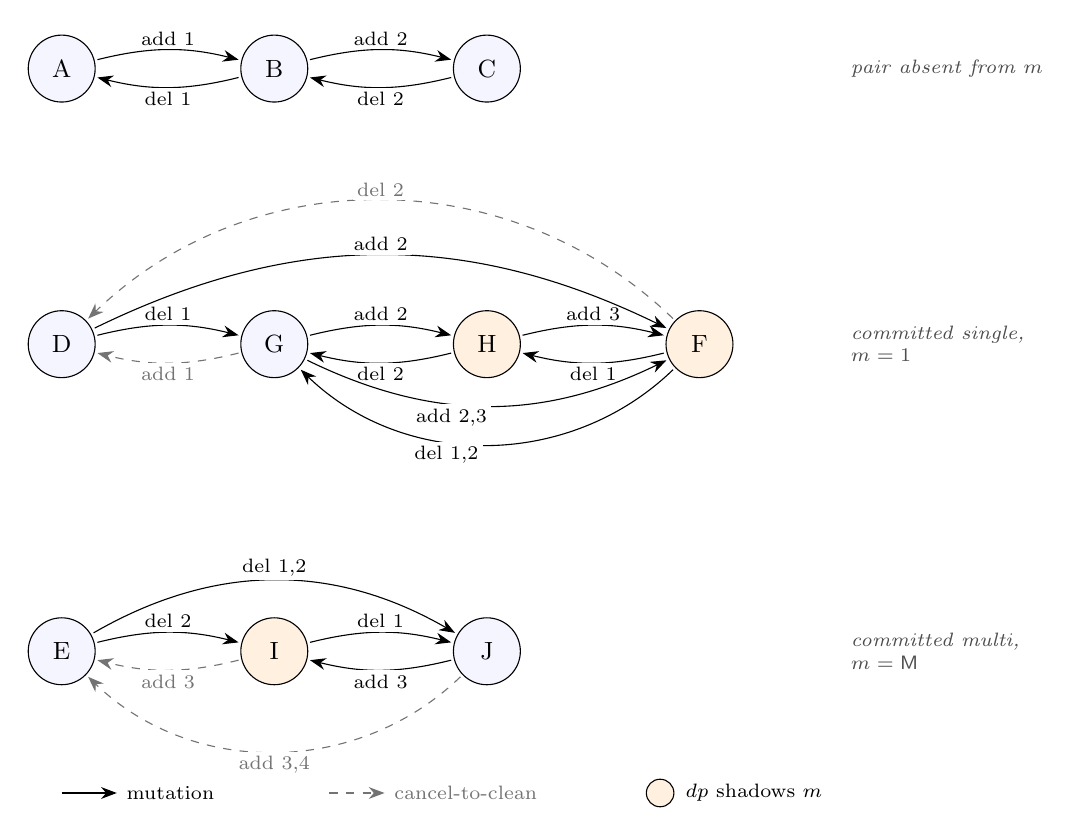
\begin{tikzpicture}[
  font=\small,
  st/.style={draw,circle,minimum size=8.5mm,inner sep=1pt,fill=blue!4},
  sh/.style={st,fill=orange!12},
  >={Stealth[length=2mm]},
  lbl/.style={font=\scriptsize,inner sep=1.5pt,fill=white},
  ed/.style={->,shorten >=1pt,shorten <=1pt},
  cancel/.style={ed,dashed,black!55},
  band/.style={font=\scriptsize\itshape,anchor=west,align=left,black!70}
]
% ---------------- band 1: uncommitted (pair absent from m) ----------------
\node[st] (A) at (0,0)    {A};
\node[st] (B) at (2.7,0)  {B};
\node[st] (C) at (5.4,0)  {C};
\draw[ed,bend left=14]  (A) to node[lbl,above]{add 1} (B);
\draw[ed,bend left=14]  (B) to node[lbl,below]{del 1} (A);
\draw[ed,bend left=14]  (B) to node[lbl,above]{add 2} (C);
\draw[ed,bend left=14]  (C) to node[lbl,below]{del 2} (B);
\node[band] at (9.9,0) {pair absent from $m$};

% ---------------- band 2: committed single, m = 1 ----------------
\node[st] (D) at (0,-3.5)    {D};
\node[st] (G) at (2.7,-3.5)  {G};
\node[sh] (H) at (5.4,-3.5)  {H};
\node[sh] (F) at (8.1,-3.5)  {F};
\draw[ed,bend left=14]     (D) to node[lbl,above]{del 1} (G);
\draw[cancel,bend left=14] (G) to node[lbl,below]{add 1} (D);
\draw[ed,bend left=14]     (G) to node[lbl,above]{add 2} (H);
\draw[ed,bend left=14]     (H) to node[lbl,below]{del 2} (G);
\draw[ed,bend left=14]     (H) to node[lbl,above]{add 3} (F);
\draw[ed,bend left=14]     (F) to node[lbl,below]{del 1} (H);
% long arcs, both routed above
\draw[ed,bend left=26]     (D) to node[lbl,above,pos=0.5]{add 2} (F);
\draw[cancel,bend right=44](F) to node[lbl,above,pos=0.5]{del 2} (D);
% long arcs, both routed below
\draw[ed,bend right=26]    (G) to node[lbl,below,pos=0.4]{add 2,3} (F);
\draw[ed,bend left=44]     (F) to node[lbl,below,pos=0.6]{del 1,2} (G);
\node[band] at (9.9,-3.5) {committed single,\\$m = 1$};

% ---------------- band 3: committed multi, m = M ----------------
\node[st] (E) at (0,-7.4)    {E};
\node[sh] (I) at (2.7,-7.4)  {I};
\node[st] (J) at (5.4,-7.4)  {J};
\draw[ed,bend left=14]     (E) to node[lbl,above]{del 2} (I);
\draw[cancel,bend left=14] (I) to node[lbl,below]{add 3} (E);
\draw[ed,bend left=14]     (I) to node[lbl,above]{del 1} (J);
\draw[ed,bend left=14]     (J) to node[lbl,below]{add 3} (I);
\draw[ed,bend left=30]     (E) to node[lbl,above,pos=0.5]{del 1,2} (J);
\draw[cancel,bend left=44] (J) to node[lbl,below,pos=0.5]{add 3,4} (E);
\node[band] at (9.9,-7.4) {committed multi,\\$m = \M$};

% ---------------- legend ----------------
\draw[->,black]           (0,-9.2) -- (0.7,-9.2)
  node[right,font=\scriptsize]{mutation};
\draw[->,dashed,black!55] (3.4,-9.2) -- (4.1,-9.2)
  node[right,font=\scriptsize]{cancel-to-clean};
\node[draw,circle,fill=orange!12,minimum size=3.5mm,inner sep=0pt] at (7.6,-9.2) {};
\node[right,font=\scriptsize] at (7.8,-9.2) {$dp$ shadows $m$};
\end{tikzpicture}
\caption{Per-pair transitions. Dashed edges are
Invariant~\ref{inv:cancel} at work: an operation that restores the pair's
committed value \emph{removes} deltas rather than adding a shadow. Shaded
states are those where $dp$ and $m$ hold the same pair with different values
--- impossible in a Boolean delta matrix, and the reason the iterator needs a
shadow rule.}
\label{fig:automaton}
\end{figure}

Reading the diagram: the three horizontal bands are the pair's committed
status, which a transaction cannot change, so no transition here crosses bands.
Within a band, adding and removing identifiers moves left and right, and every
cycle returns to the canonical state --- $\mathbf{D}
\xrightarrow{\text{add}} \mathbf{F} \xrightarrow{\text{del}} \mathbf{D}$
leaves no residue, which is exactly what Invariant~\ref{inv:cancel} demands.

The one operation that \emph{does} change committed status is folding, and it is
therefore the only thing that moves a pair between bands. It is left out of this
figure on purpose --- it is not a mutation, and no query can observe it --- and
drawn on its own in Figure~\ref{fig:fold}, discussed in \S\ref{sec:folding}.

% =====================================================================
\section{Algorithms}
\label{sec:algorithms}

\subsection{Point reads}
\label{sec:reads}

\begin{algorithm}[H]
\caption{Effective read and identifier enumeration}
\label{alg:get}
\begin{algorithmic}[1]
\Function{EffGet}{$s,d$}
  \State \Call{WaitFwd}{} \Comment{materialise $dp,dm$; $m$ is never pending (\S\ref{sec:hazard-resize})}
  \If{$dp$ has $(s,d)$}
    \State \Return $dp(s,d)$
  \EndIf
  \If{$|dm| \neq 0$ \textbf{and} $dm$ has $(s,d)$}
    \State \Return $\bot$ \Comment{deleted}
  \EndIf
  \State \Return $m(s,d)$ \Comment{possibly $\bot$}
\EndFunction
\Statex
\Function{Get}{$s,d$} \Comment{returns an owned iterator}
  \State $v \gets \Call{EffGet}{s,d}$
  \If{$v = \M$}
    \State \Return \Call{RowScan}{$me,\ \kappa(s,d)$} \Comment{ascending identifier order}
  \Else
    \State \Return \Call{AtMostOne}{$v$} \Comment{no allocation}
  \EndIf
\EndFunction
\end{algorithmic}
\end{algorithm}

Algorithm~\ref{alg:get} gives both, and Appendix~\ref{app:table} tabulates
$\varepsilon$'s four cases against the layers directly.
The single-edge path costs at most three FFI lookups and \emph{no}
allocation: the returned iterator is an \texttt{Option} iterator by value.
This matters because \textsc{Get} is the inner loop of the query operators
that resolve a bound $(s,d)$ pair to concrete edges --- \texttt{ExpandInto}
and the bound-destination case of \texttt{CondTraverse} call it once per
candidate pair. The $|dm| \neq 0$ test before probing $dm$ is a
micro-optimisation with macro consequences: on a read-only workload against a
freshly loaded graph, $dm$ is empty, and skipping the probe removes an FFI
call from the hottest path in the engine.

\subsection{Bulk insertion}
\label{sec:insert}

Insertion is where the host runtime's non-blocking semantics dictate program
structure. The naive loop --- for each edge, read the pair's current state,
then write --- interleaves reads and writes of $dp$. Every write leaves $dp$
pending; every subsequent read must materialise it. With $n$ edges that is
$\Theta(n)$ materialisations, each at least linear in the accumulated delta:
\emph{quadratic} bulk insertion. The artifact therefore splits the operation
into a read phase that touches $dp$ only for reading and a write phase that
touches it only for writing (Algorithm~\ref{alg:insert}).

\begin{algorithm}[!ht]
\small
\caption{\textsc{SetAllFromSlices}: bulk insert with in-batch promotion}
\label{alg:insert}
\begin{algorithmic}[1]
\Require parallel slices $\mathit{srcs}, \mathit{dsts}, \mathit{ids}$ of length $n$
\State \Call{WaitFwd}{}; \ $\mathit{dmEmpty} \gets (|dm| = 0)$
\State $\mathit{batch} \gets$ empty hash map $(s,d) \mapsto$ slot index
\State $Q \gets$ empty list of $(s, d, \mathit{val}, \mathit{committed})$ \Comment{queued inline writes}
\Statex \textit{// ---- read phase: decide placement; write only to $me$ ----}
\For{$(s,d,e)$ in the input}
  \State $k \gets \kappa(s,d)$
  \If{$(s,d) \in \mathit{batch}$}
    \State $i \gets \mathit{batch}[(s,d)]$
    \If{$i \neq \textsc{marked}$} \Comment{2nd edge of a pair new in this batch}
      \State $me[k,\, Q[i].\mathit{val}] \gets \mathrm{true}$;\quad $Q[i].\mathit{val} \gets \M$
      \State $\textit{multi} \gets \textit{multi} + 1$;\quad $\mathit{batch}[(s,d)] \gets \textsc{marked}$
    \EndIf
    \State $me[k,e] \gets \mathrm{true}$
  \Else
    \State $\mathit{masked} \gets \lnot \mathit{dmEmpty} \wedge dm \text{ has } (s,d)$
    \State $\mathit{fromDp} \gets dp(s,d)$
    \State $\mathit{cur} \gets \mathit{fromDp}$ if present, else ($\bot$ if $\mathit{masked}$, else $m(s,d)$)
    \If{$\mathit{cur} = \M$} \Comment{already multi-edge}
      \State $me[k,e] \gets \mathrm{true}$;\ \ $\mathit{batch}[(s,d)] \gets \textsc{marked}$
    \ElsIf{$\mathit{cur} \neq \bot$} \Comment{promote an existing single edge}
      \State $me[k, \mathit{cur}] \gets \mathrm{true}$;\ \ $me[k,e] \gets \mathrm{true}$;\ \ $\textit{multi} \gets \textit{multi} + 1$
      \State $\mathit{batch}[(s,d)] \gets \textsc{marked}$
      \State append $(s,d,\M,\ m(s,d)$ if $\mathit{fromDp}$ present else $\bot)$ to $Q$
    \Else \Comment{first edge for this pair: inline}
      \State $\mathit{batch}[(s,d)] \gets |Q|$
      \State append $(s,d,e,\ m(s,d)$ if $\mathit{masked}$ else $\bot)$ to $Q$
    \EndIf
  \EndIf
\EndFor
\Statex \textit{// ---- write phase: inline values into $dp$, structure into $mt$ ----}
\For{$(s,d,\mathit{val},\mathit{committed})$ in $Q$}
  \State $mt[d,s] \gets \mathrm{true}$
  \If{$\mathit{committed} \neq \bot$}
    \State remove $(s,d)$ from $dm$ \Comment{restore Invariant~\ref{inv:pure}}
    \If{$\mathit{committed} = \mathit{val}$}
      \State remove $(s,d)$ from $dp$;\ \ \textbf{continue}
        \Comment{cancel to clean, Invariant~\ref{inv:cancel}}
    \EndIf
  \EndIf
  \State $dp[s,d] \gets \mathit{val}$
\EndFor
\end{algorithmic}
\end{algorithm}

Three details carry the weight.

\paragraph{$me$ may be written during the read phase.}
The phase split is not ``no writes then all writes''; it is ``no writes
\emph{to matrices this phase reads}''. $me$ is never read here --- promotion
decisions are made from the inline value alone, by
Invariant~\ref{inv:promotion} --- so its pending work is harmless and can
accumulate into one bulk build.

\paragraph{In-batch duplicates need retroactive promotion.}
A batch may contain two edges for the same previously-absent pair. When the
first is seen, its identifier is queued for the inline slot; when the second
arrives, that queued slot is rewritten to $\M$ \emph{in place} and the
already-queued identifier is pushed to $me$. The $\mathit{batch}$ map exists
exactly to make this possible, and the \textsc{marked} sentinel
(\texttt{usize::MAX} in the artifact) distinguishes ``this pair has a pending
inline slot at index $i$'' from ``this pair is already multi-edge, send
further identifiers straight to $me$''.

\paragraph{Delta reconciliation is deferred to the write phase.}
The read phase records, per queued pair, the \emph{committed} value it will
need to reconcile against: for a $dm$-masked pair, so the write phase can
clear the mask (Invariant~\ref{inv:pure}); and for a $dp$-shadowed pair being
promoted, because that pair may have $m = \M$ already --- it was demoted
earlier in the same transaction --- in which case re-promotion must
\emph{cancel} the shadow rather than write $dp = \M$ over $m = \M$
(Invariant~\ref{inv:cancel}). This is the $\mathbf{I} \to \mathbf{E}$ dashed
edge of Figure~\ref{fig:automaton}.

\begin{proposition}[Cost]
\label{prop:insertcost}
Algorithm~\ref{alg:insert} performs $O(n)$ FFI calls, $O(1)$ matrix
materialisations, and $O(n)$ expected hash operations, with $O(n)$ auxiliary
memory.
\end{proposition}
\begin{proof}
\textsc{WaitFwd} is called once. The read phase makes at most three point
probes ($dm$, $dp$, $m$) and at most two $me$ writes per input element and no
call that reads $dp$ or $dm$ after the wait; the write phase makes at most
three writes per queued element and never reads them. No point read of a
matrix follows a write to that same matrix, so no further materialisation is
triggered. Hash operations are one \texttt{entry} lookup per element,
expected $O(1)$.
\end{proof}

\subsection{Bulk deletion}
\label{sec:delete}

Deletion has a fast path chosen by a single test, $|me| \neq 0$
(\textsc{HasMultiEdge}). If \emph{no} pair in the tensor is multi-edge, every
edge is its pair's inline value, so removing a set of edges is removing a set
of pairs --- expressible in three bulk GraphBLAS operations regardless of how
many edges are involved:

\begin{align}
  dm\langle \mathit{mask}\rangle &\mathrel{{=}} \mathit{mask} \cap m
    &&\text{(mark committed cells deleted)} \label{eq:dmmask}\\
  dp &\mathrel{{=}} dp \setminus \mathit{mask}
    &&\text{(drop pending adds, incl.\ shadows)} \notag\\
  mt &\mathrel{{=}} \text{\textsc{RemoveMask}}(mt, \mathit{mask}^{\!\top})
    &&\text{(same layer math, Boolean)} \notag
\end{align}

Equation~\eqref{eq:dmmask} is implemented with \texttt{eWiseMult} over
\texttt{ANY\_PAIR\_BOOL} and \emph{not} with a masked \texttt{eWiseAdd} copy;
\S\ref{sec:hazard-zero} explains why that is a correctness requirement rather
than a style preference. Removing pending adds in the same sweep is what
keeps Invariant~\ref{inv:pure} true: a pair in state $\mathbf{H}$ or
$\mathbf{F}$ has both a $dp$ shadow and a live $m$ cell, and the two
operations together move it to $\mathbf{G}$.

The slow path (Algorithm~\ref{alg:remove}) is per-edge and is the only place
demotion happens. For a
multi-edge pair, the identifier is removed from $me$ and the row is then
probed for \emph{at most two} survivors --- enough to distinguish ``still
multi'', ``exactly one left, demote'', and ``empty, delete the pair'' without
counting the row:

\begin{algorithm}[H]
\caption{\textsc{RemoveAll}, slow path (per edge $(e,s,d)$)}
\label{alg:remove}
\begin{algorithmic}[1]
\State $k \gets \kappa(s,d)$
\Switch{\Call{EffGet}{$s,d$}}
  \Case{$\M$}
    \State remove column $e$ from row $k$ of $me$
    \State $\mathit{survivor} \gets$ first entry of row $k$ (or $\bot$)
    \State $\mathit{stillMulti} \gets$ a second entry of row $k$ exists
    \If{$\mathit{stillMulti}$}
      \State \Return \Comment{no state change}
    \EndIf
    \State $\textit{multi} \gets \textit{multi} - 1$
    \If{$\mathit{survivor} \neq \bot$} \Comment{demote: it returns inline}
      \State remove column $\mathit{survivor}$ from row $k$ of $me$
      \If{$m(s,d) = \mathit{survivor}$}
        \State remove $(s,d)$ from $dp$ \Comment{cancel to clean}
      \Else
        \State $dp[s,d] \gets \mathit{survivor}$ \Comment{shadow $m$}
      \EndIf
    \Else \Comment{row emptied: the pair is gone}
      \State remove $(s,d)$ from $dp$
      \If{$m$ has $(s,d)$} \State $dm[s,d] \gets \mathrm{true}$ \EndIf
      \State remove $(d,s)$ from $mt$;\ \ report $(s,d)$ emptied
    \EndIf
  \EndCase
  \Case{$e$ --- the inline value matches}
    \State remove $(s,d)$ from $dp$
    \If{$m$ has $(s,d)$} \State $dm[s,d] \gets \mathrm{true}$ \EndIf
    \State remove $(d,s)$ from $mt$;\ \ report $(s,d)$ emptied
  \EndCase
  \Case{otherwise} \Comment{unknown identifier, or absent pair}
    \State \Return
  \EndCase
\EndSwitch
\end{algorithmic}
\end{algorithm}

The returned list of emptied pairs is the interface to the graph-wide
adjacency matrix, which is the union over relationship types: a pair is
removed from it only if it is empty in \emph{every} tensor, so the caller
intersects this report across types.

\begin{remark}[An asymmetry worth naming]
The fast path reports \emph{all} input pairs as emptied without verifying
that the supplied identifier is the pair's inline value; the slow path
reports only pairs it actually emptied. The asymmetry is sound given how the
method is called --- callers derive the removal list from the tensor itself,
by scanning it for edges incident to deleted nodes or by resolving bound
edges --- so a supplied identifier that does not match is not a case that
arises. It is nonetheless a precondition of the fast path that is documented
rather than checked, and the kind of thing that a future caller with a
different provenance for its removal list could violate quietly.
\end{remark}

\subsection{Iteration}
\label{sec:iter}

Iteration composes a three-way sorted merge over the forward layers with a
per-pair row scan of $me$. The merge exploits the fact that GraphBLAS row
iterators yield ascending $(\mathit{row}, \mathit{col})$ order, so no sorting
or intermediate materialisation is needed; $dm$ is consumed as a lookahead
that drops matching $m$ entries, and a $dp$ entry at the same position as an
$m$ entry wins and \emph{suppresses} it --- the shadow rule. Both delta
iterators are elided entirely when their layer is empty, which on a
read-mostly workload avoids allocating and freeing two \texttt{GxB\_Iterator}
objects per scan.

\begin{figure}[t]
\centering
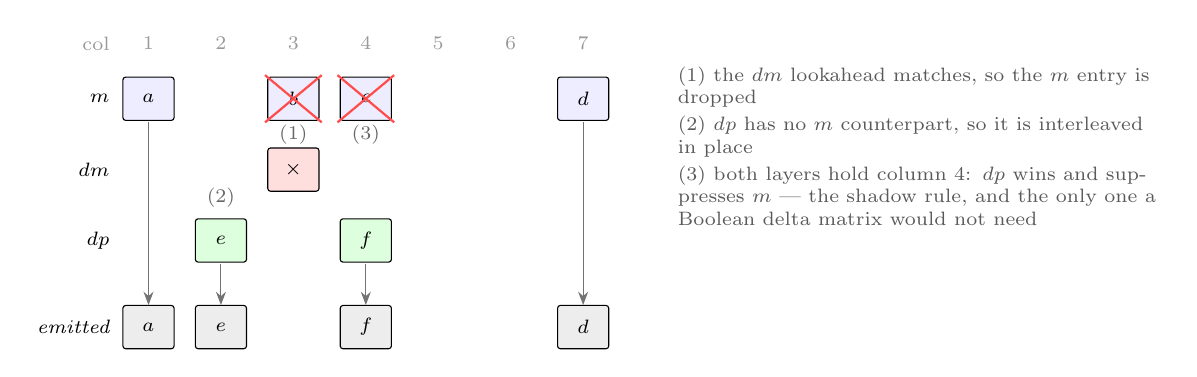
\begin{tikzpicture}[
  font=\small,
  cell/.style={draw,minimum width=6.5mm,minimum height=5.5mm,inner sep=0pt,
               font=\scriptsize,rounded corners=1pt},
  mc/.style={cell,fill=blue!7},
  pc/.style={cell,fill=green!13},
  dc/.style={cell,fill=red!13},
  oc/.style={cell,fill=black!7},
  rl/.style={font=\scriptsize\itshape,anchor=east},
  nt/.style={font=\scriptsize,align=center,black!65,inner sep=1pt}
]
\def\X{0.92}
\def\LX{7.6}
% column ruler
\foreach \c in {1,...,7} {\node[font=\scriptsize,black!40] at (\c*\X,0.70) {\c};}
\node[font=\scriptsize,black!40,anchor=east] at (0.55,0.70) {col};
% layers
\node[rl] at (0.55,0)     {$m$};
\node[mc] at (1*\X,0)  {$a$};  \node[mc] at (3*\X,0)  {$b$};
\node[mc] at (4*\X,0)  {$c$};  \node[mc] at (7*\X,0)  {$d$};
\node[rl] at (0.55,-0.9)  {$dm$};
\node[dc] at (3*\X,-0.9) {$\times$};
\node[rl] at (0.55,-1.8)  {$dp$};
\node[pc] at (2*\X,-1.8) {$e$};  \node[pc] at (4*\X,-1.8) {$f$};
% output
\node[rl] at (0.55,-2.9)  {emitted};
\node[oc] at (1*\X,-2.9) {$a$};  \node[oc] at (2*\X,-2.9) {$e$};
\node[oc] at (4*\X,-2.9) {$f$};  \node[oc] at (7*\X,-2.9) {$d$};
% provenance
\draw[->,black!55,>=Stealth] (1*\X,-0.30) -- (1*\X,-2.62);
\draw[->,black!55,>=Stealth] (7*\X,-0.30) -- (7*\X,-2.62);
\draw[->,black!55,>=Stealth] (2*\X,-2.10) -- (2*\X,-2.62);
\draw[->,black!55,>=Stealth] (4*\X,-2.10) -- (4*\X,-2.62);
% struck cells: m@3 deleted by the dm lookahead, m@4 suppressed by dp@4
\draw[red!70,thick] (3*\X-0.36,0.30) -- (3*\X+0.36,-0.30);
\draw[red!70,thick] (3*\X+0.36,0.30) -- (3*\X-0.36,-0.30);
\draw[red!70,thick] (4*\X-0.36,0.30) -- (4*\X+0.36,-0.30);
\draw[red!70,thick] (4*\X+0.36,0.30) -- (4*\X-0.36,-0.30);
% call-outs
\node[font=\scriptsize,black!60] at (3*\X,-0.45) {(1)};
\node[font=\scriptsize,black!60] at (2*\X,-1.25) {(2)};
\node[font=\scriptsize,black!60] at (4*\X,-0.45) {(3)};
% legend, clear of the diagram
\node[nt,anchor=north west,text width=6.2cm,align=left] at (\LX,0.45)
  {(1) the $dm$ lookahead matches, so the $m$ entry is dropped\\[2pt]
   (2) $dp$ has no $m$ counterpart, so it is interleaved in place\\[2pt]
   (3) both layers hold column 4: $dp$ wins and suppresses $m$ ---
       the shadow rule, and the only one a Boolean delta matrix
       would not need};
\end{tikzpicture}
\caption{One row of the three-way merge. The three layer iterators are already
ascending, so the merge is a single pass with two lookaheads and no
intermediate matrix: a $dm$ entry deletes the $m$ entry it matches (column 3), a
$dp$ entry with no $m$ counterpart is interleaved (column 2), and a $dp$ entry at
an occupied column wins (column 4) --- which is the only rule a Boolean delta
matrix would not need. The emitted row is the effective state
$(m \setminus dm) \cup dp$, in ascending column order, each entry once.}
\label{fig:merge}
\end{figure}

Two orientations are supported. Forward iteration streams inline values
directly. Backward iteration streams the Boolean structure of $mt$ and
recovers each pair's inline value with \textsc{EffGet}, paying one point
lookup per incoming pair --- the deliberate consequence of not storing
identifiers twice (\S\ref{sec:representation}).

A separate whole-tensor enumeration, \textsc{IterEdges}, exists for
consumers that need every edge but not in pair order (snapshot writing, index
rebuilds). It concatenates the forward stream with sentinels filtered out and
a single flat scan of $me$, unpacking $\kappa$ back into $(s,d)$ by shifting.
On a simple graph $me$ is empty and this degenerates to one streaming pass
with no sub-iterator at all --- the point of the whole design, visible in one
line of code.

\subsection{Folding}
\label{sec:folding}

Folding merges an oversized delta into the base. For the Boolean layers the
usual pattern union suffices; for the \texttt{UINT64} forward layer it must
be \emph{value-preserving and $dp$-favouring}, because a shadowed pair's live
value is in $dp$:
\[
  m \mathrel{{=}} m \oplus_{\textsc{second}} dp, \qquad dp \mathrel{{=}} \emptyset;
  \qquad\quad m \mathrel{{=}} m \setminus dm, \qquad dm \mathrel{{=}} \emptyset .
\]
\textsc{Second} makes $dp$ win on the intersection, which is exactly the
shadow semantics. By Invariant~\ref{inv:pure} the two folds are
order-independent, so each layer carries its own decision.

\begin{figure}[t]
\centering
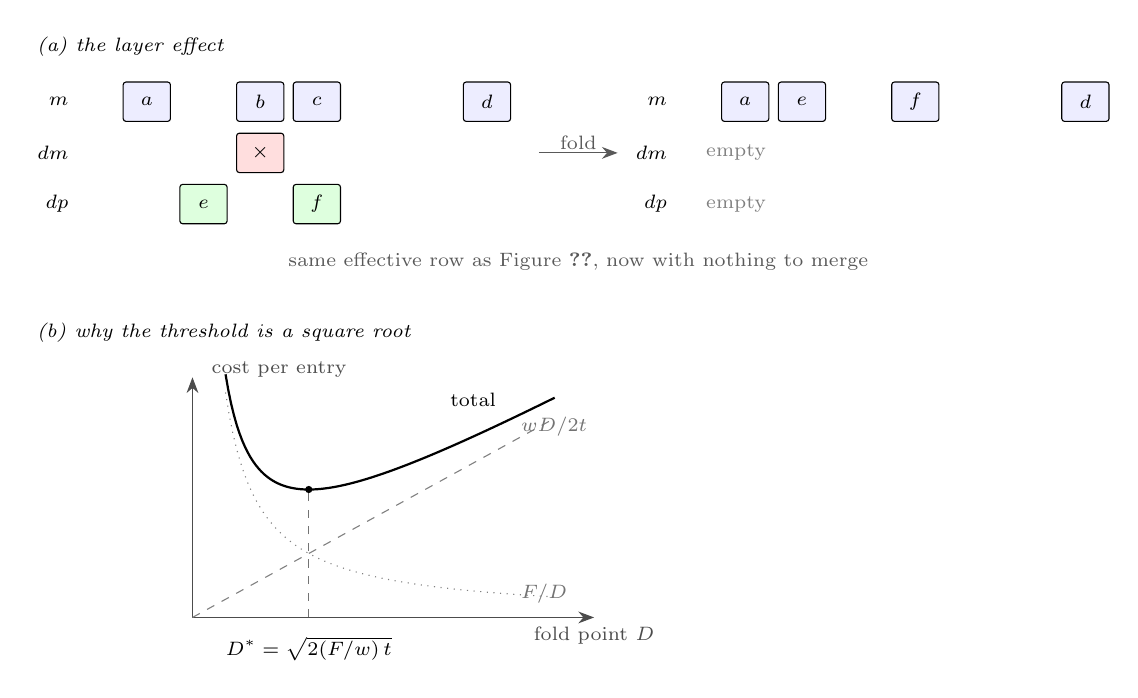
\begin{tikzpicture}[
  font=\small,
  cell/.style={draw,minimum width=6mm,minimum height=5mm,inner sep=0pt,
               font=\scriptsize,rounded corners=1pt},
  mc/.style={cell,fill=blue!7},
  pc/.style={cell,fill=green!13},
  dc/.style={cell,fill=red!13},
  rl/.style={font=\scriptsize\itshape,anchor=east},
  >={Stealth[length=2mm]}
]
\def\X{0.72}
% ---- (a) what the fold does to the layers, on Figure 4's example ----
\node[font=\scriptsize\itshape,anchor=west] at (0.1,1.15) {(a) the layer effect};
\node[rl] at (0.75,0.45)   {$m$};
\node[mc] at (1*\X+0.9,0.45) {$a$}; \node[mc] at (3*\X+0.9,0.45) {$b$};
\node[mc] at (4*\X+0.9,0.45) {$c$}; \node[mc] at (7*\X+0.9,0.45) {$d$};
\node[rl] at (0.75,-0.2)   {$dm$};
\node[dc] at (3*\X+0.9,-0.2) {$\times$};
\node[rl] at (0.75,-0.85)  {$dp$};
\node[pc] at (2*\X+0.9,-0.85) {$e$}; \node[pc] at (4*\X+0.9,-0.85) {$f$};
\draw[->,black!65] (6.6,-0.2) -- (7.6,-0.2)
  node[midway,above,font=\scriptsize,align=center,inner sep=1pt]{fold};
\node[rl] at (8.35,0.45)   {$m$};
\node[mc] at (1*\X+8.5,0.45) {$a$}; \node[mc] at (2*\X+8.5,0.45) {$e$};
\node[mc] at (4*\X+8.5,0.45) {$f$}; \node[mc] at (7*\X+8.5,0.45) {$d$};
\node[rl] at (8.35,-0.2)   {$dm$};
\node[font=\scriptsize,black!50,anchor=west] at (8.6,-0.2) {empty};
\node[rl] at (8.35,-0.85)  {$dp$};
\node[font=\scriptsize,black!50,anchor=west] at (8.6,-0.85) {empty};
\node[font=\scriptsize,black!65,anchor=north,align=center] at (7.1,-1.35)
  {same effective row as Figure~\ref{fig:merge}, now with nothing to merge};

% ---- (b) the cost trade-off ----
\begin{scope}[yshift=-6.1cm,xshift=2.2cm]
  \node[font=\scriptsize\itshape,anchor=west] at (-2.1,3.62)
    {(b) why the threshold is a square root};
  \node[font=\scriptsize,black!70,anchor=west] at (0.12,3.15) {cost per entry};
  \draw[->,black!70] (0,0) -- (5.1,0) node[below,font=\scriptsize]{fold point $D$};
  \draw[->,black!70] (0,0) -- (0,3.05);
  % rewrite tax  c*D, c = 0.55
  \draw[domain=0.0:4.6,samples=40,black!50,dashed] plot (\x,{0.55*\x});
  \node[font=\scriptsize,black!55,anchor=west] at (4.05,2.42) {$wD/2t$};
  % fold bill F/D, F = 1.2
  \draw[domain=0.42:4.6,samples=90,black!50,dotted] plot (\x,{1.2/\x});
  \node[font=\scriptsize,black!55,anchor=west] at (4.05,0.30) {$F/D$};
  % total
  \draw[domain=0.42:4.6,samples=120,thick,black] plot (\x,{0.55*\x + 1.2/\x});
  \node[font=\scriptsize,anchor=south west] at (3.15,2.55) {total};
  % minimum
  \draw[dashed,black!55] (1.477,0) -- (1.477,1.625);
  \fill (1.477,1.625) circle (1.3pt);
  \node[font=\scriptsize,anchor=north,align=center] at (1.477,-0.12)
    {$D^{\ast}=\sqrt{2(F/w)\,t}$};
\end{scope}
\end{tikzpicture}
\caption{Folding. (a) Both deltas are merged into the base and cleared; readers
see the same effective row before and after, which is why a fold is invisible
(Figure~\ref{fig:fold} is the same statement at the level of states). (b) The
two costs pull in opposite directions --- a delta left to grow taxes every later
transaction, a delta folded too eagerly pays the fixed fold cost too often ---
and their sum is least where they cross. That the crossing is at
$\sqrt{2(F/w)t}$ rather than at a constant is the whole reason the rule depends
on transaction size; the minimum is now machine-checked
(\S\ref{sec:mechanised}).}
\label{fig:foldcost}
\end{figure}

\paragraph{When to fold.} A fixed threshold is the obvious rule and the wrong
one. The premise that sets the shape is that \emph{every write transaction
pays $O(|\delta|)$}, not $O(\text{what it added})$: it copy-on-write dups the
delta and, if anything materialises it, merges its pending tuples. So with
transactions of $t$ entries accumulating to a fold point $D$, writing $D$
entries costs $\sum_i (i\,t)\,w + F \approx wD^2/(2t) + F$, i.e.\ per entry
$wD/(2t) + F/D$ --- a rewrite tax growing with $D$ against a fold bill
shrinking with it. The two balance at
\[
  D^{\ast} \;=\; \sqrt{2\,(F/w)\,t} ,
\]
which is why this is a square-root rule rather than the LSM-style ratio
$D \ge \text{base}/K$. Figure~\ref{fig:foldcost}(b) draws the two terms and
their crossing. A ratio is right when each entry is rewritten $O(1)$
times between merges; here every transaction re-touches the \emph{whole}
delta, so the accumulated tax is quadratic in $D$ and depends on $t$.

$F$ and $w$ are measured rather than modelled. Two properties of $F$ are what
let the rule ignore the base. It is independent of $\mathrm{nrows}$: an empty
fold costs $2.0$--$2.5\,\mu\text{s}$ at $\mathrm{nrows} = 65\text{k}$,
$1\text{M}$ and $16.7\text{M}$ alike, which is the measurement that retired an
earlier policy's $\mathrm{nvals} + \mathrm{nrows}$ base term. And against
$\mathrm{nvals}$ it is strongly \emph{sub}-linear --- $\approx\!2\,\mu\text{s}$
empty, $707\,\mu\text{s}$ at $16\text{k}$ ($43$\,ns/entry),
$2{,}174\,\mu\text{s}$ at $1\text{M}$ ($2$\,ns/entry) --- which is two format
regimes rather than one line, since a delta at $1.5\%$ density is hypersparse
and one at $95\%$ is sparse or bitmap, and \texttt{eWiseAdd} vectorises only in
the latter. Fitting a straight line across that curve yields an apparent fixed
cost of $\approx\!1.7$\,ms, and we flag it as an artifact of the regime change
rather than a constant term, because a policy calibrated on it would be
calibrated on a fit. What the rule actually needs is $F$ near the operating
point, and there it moves $1.2\times$ for $4\times$ the entries between $262$k
and $1$M --- flat enough that the balance point does not track base size. And
$w$ differs by
$250\times$ between the two paths: a write nobody reads pays only the dup
($w_{\text{dup}} \approx 0.2\,\text{ns}$/entry, memcpy speed), while a
transaction whose delta is also materialised pays the pending-tuple merge
($w_{\text{merge}} \approx 50\,\text{ns}$/entry). Since
$D^{\ast} \propto 1/\sqrt{w}$, the read path's balance point sits
$\sqrt{250} \approx 16\times$ tighter than the write path's, and the artifact
uses separate constants accordingly.

One escape hatch overrides the balance point: a delta comparable to the base
($2|\delta| \ge |m|$) always folds, because the fold then costs the same order
as a single delta touch and because the delta is holding as much memory as the
base it shadows. Without it a one-shot bulk transaction --- whose huge $t$
defeats the square-root term --- can leave a base-sized delta taxing every
later transaction, and a delete-everything leaves the tensor holding $m$ and a
tombstone set of equal size until something happens to touch that matrix
again.

\paragraph{Where the decision is taken, and why it is not a correctness
concern.} The decision is \emph{latched} at version creation and at reads, but
\emph{executed} before the next mutation, where folding also replaces the
copy-on-write dup of both the delta and the base. Deliberately, a read does not
schedule its own fold: a create-then-delete transaction would otherwise fold
its own pending additions into the base immediately before deleting them,
leaving the base full of stale entries and the tombstone set full of
tombstones that later transactions erode one at a time.

All of this is throughput policy, and it is worth being explicit that it is
\emph{only} throughput policy. The sizes it consults are approximate counters
maintained without GraphBLAS calls --- reading a delta's true \texttt{nvals}
would force its pending tuples to merge, the very $O(|\delta|)$ cost the policy
exists to bound --- so they drift, and by design. Folding preserves the
effective state pointwise, so no choice of constants and no drift in the
counters can change what the tensor denotes. \S\ref{sec:mechanised} states
that as a theorem.

\paragraph{What folding does to the automaton.} Folding is the only transition
that moves a pair between the three bands of Figure~\ref{fig:automaton}, because
it is the only operation that changes a pair's \emph{committed} status. It is
also the only transition that is not a mutation: it is invisible to readers
(\S\ref{sec:mechanised}), so it is drawn separately, in
Figure~\ref{fig:fold}.

Folding $dp$ commits whatever the pending layer holds --- promoting the two
uncommitted states and collapsing all three shadowed ones:
\[
  \mathbf{B} \to \mathbf{D}, \quad
  \mathbf{C} \to \mathbf{E}, \quad
  \mathbf{H} \to \mathbf{D}, \quad
  \mathbf{F} \to \mathbf{E}, \quad
  \mathbf{I} \to \mathbf{D} .
\]
Folding $dm$ applies the tombstones, which removes the pair outright:
$\mathbf{G} \to \mathbf{A}$ and $\mathbf{J} \to \mathbf{A}$. On
$\{\mathbf{A}, \mathbf{D}, \mathbf{E}\}$ both folds are the identity, since
those are exactly the states with no deltas to fold.

Two things are worth reading off that. First, the map is total and its image is
$\{\mathbf{A}, \mathbf{D}, \mathbf{E}\}$ --- so the ten states are a
transaction-local phenomenon and a quiescent tensor occupies only three of them.
Note this needs $\mathbf{B} \to \mathbf{D}$ and $\mathbf{C} \to \mathbf{E}$: a
pair whose edges were all created in the current transaction is uncommitted, not
shadowed, and it is folding $dp$ that makes it committed. Second, the shadowed
states $\mathbf{F}, \mathbf{H}, \mathbf{I}$ have no preimage under the map, which
is another way of saying that shadowing is something only a live transaction can
produce.

\begin{figure}[t]
\centering
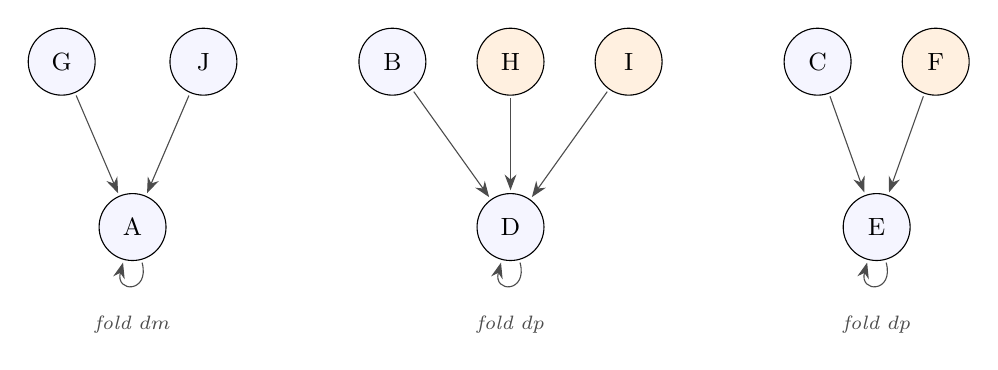
\begin{tikzpicture}[
  font=\small,
  st/.style={draw,circle,minimum size=8.5mm,inner sep=1pt,fill=blue!4},
  sh/.style={st,fill=orange!12},
  >={Stealth[length=2mm]},
  fd/.style={->,shorten >=1pt,shorten <=1pt,black!70},
  lbl/.style={font=\scriptsize,inner sep=1.5pt,fill=white}
]
% sources, grouped over their image
\node[st] (G) at (-0.9,0)  {G};
\node[st] (J) at (0.9,0)   {J};
\node[st] (B) at (3.3,0)   {B};
\node[sh] (H) at (4.8,0)   {H};
\node[sh] (I) at (6.3,0)   {I};
\node[st] (C) at (8.7,0)   {C};
\node[sh] (F) at (10.2,0)  {F};
% images
\node[st] (A) at (0,-2.1)    {A};
\node[st] (D) at (4.8,-2.1)  {D};
\node[st] (E) at (9.45,-2.1) {E};
% fold dm: apply the tombstones
\draw[fd] (G) -- (A);
\draw[fd] (J) -- (A);
% fold dp: commit the pending layer
\draw[fd] (B) -- (D);
\draw[fd] (H) -- (D);
\draw[fd] (I) -- (D);
\draw[fd] (C) -- (E);
\draw[fd] (F) -- (E);
% identity on the quiescent states
\draw[fd] (A) to[loop below,looseness=5] (A);
\draw[fd] (D) to[loop below,looseness=5] (D);
\draw[fd] (E) to[loop below,looseness=5] (E);
% band labels
\node[font=\scriptsize\itshape,black!70,anchor=north] at (0,-3.1)    {fold $dm$};
\node[font=\scriptsize\itshape,black!70,anchor=north] at (4.8,-3.1)  {fold $dp$};
\node[font=\scriptsize\itshape,black!70,anchor=north] at (9.45,-3.1) {fold $dp$};
\end{tikzpicture}
\caption{The fold map, which Figure~\ref{fig:automaton} deliberately omits
because it is not a mutation and is the only transition that crosses that
figure's bands. It is total, idempotent, and its image is
$\{\mathbf{A},\mathbf{D},\mathbf{E}\}$ --- the three states with no deltas, on
which it acts as the identity (self-loops). The shaded states are the shadowed
ones; that none of them is in the image is exactly the statement that only a
live transaction can produce a shadow.}
\label{fig:fold}
\end{figure}

\subsection{Rebuilding the transpose}
\label{sec:rebuild}

$mt$ must equal the transpose of the effective forward \emph{structure}
(Invariant~\ref{inv:mt}). It is tempting to transpose the three forward
layers into $mt$'s three layers separately, and wrong: a shadowed pair
appears in both $m$ and $dp$, and the Boolean $mt$ layers are required to be
disjoint. The artifact instead materialises $(m \setminus dm) \cup dp$ as a
Boolean matrix and transposes \emph{that} into a clean base with empty
deltas. The materialisation itself must use a pattern-only apply rather than
a valued union, for the reason in \S\ref{sec:hazard-zero}.

% =====================================================================
\section{Correctness}
\label{sec:correctness}

\begin{theorem}[Cardinality identity]
\label{thm:count}
Under Invariants~\ref{inv:masksub}--\ref{inv:counter},
\[
  |E| \;=\; \underbrace{|m| + |dp| - |dm| - |dp \cap m|}_{|P^{\ast}|}
            \;-\; \textit{multi} \;+\; |me| ,
\]
where $|dp \cap m|$ is the size of the structural intersection of $dp$ and
$m$. All six quantities are $O(1)$ GraphBLAS metadata reads except
$|dp \cap m|$, which is one \texttt{eWiseMult} over
\texttt{ANY\_PAIR\_BOOL} and is skipped entirely when $|dp| = 0$.
\end{theorem}

\begin{proof}
\emph{Pattern size.} By Definition~\ref{def:eff},
$P^{\ast} = \dom(dp) \cup (\dom(m) \setminus dm)$. By
Invariant~\ref{inv:masksub} $dm \subseteq \dom(m)$, so
$|\dom(m) \setminus dm| = |m| - |dm|$; by Invariant~\ref{inv:pure}
$\dom(dp) \cap dm = \emptyset$, so the union's inclusion--exclusion term is
$|\dom(dp) \cap (\dom(m)\setminus dm)| = |\dom(dp) \cap \dom(m)| = |dp \cap m|$.
Hence $|P^{\ast}| = |dp| + |m| - |dm| - |dp \cap m|$.

\emph{Edges per pair.} Each $p \in P^{\ast}$ contributes $|\mathrm{Ids}(p)|$
edges. If $\varepsilon(p) \neq \M$ that is $1$. If $\varepsilon(p) = \M$ it is
the number of entries in row $\kappa(p)$ of $me$, and by
Invariant~\ref{inv:promotion} those rows are non-empty exactly for such $p$
and empty for all others, so summing over $P^{\ast}$,
\[
  |E| = \bigl(|P^{\ast}| - |\{p : \varepsilon(p) = \M\}|\bigr)
        + \sum_{\varepsilon(p) = \M} |\text{row } \kappa(p)|
      = |P^{\ast}| - \textit{multi} + |me| ,
\]
using Invariant~\ref{inv:counter} for the middle term and the fact that
$\kappa$ is injective (\S\ref{sec:compound}) so the rows partition $me$.
\end{proof}

\begin{remark}
The identity is computed in \texttt{u64} arithmetic with subtractions, so a
violated invariant does not merely give a wrong count --- it can wrap.
Combined with Invariant~\ref{inv:counter}'s reliance on incremental
maintenance, this makes \texttt{edge\_count} a useful oracle: asserting it
against an independent scan is a cheap, total test of the invariant set, and
we would recommend it as a debug-mode check.
\end{remark}

\begin{theorem}[Iteration]
\label{thm:iter}
Forward iteration emits, for each $p \in P^{\ast}$ in ascending
$(\mathit{src},\mathit{dst})$ order, every element of $\mathrm{Ids}(p)$ in
ascending identifier order, each exactly once; and it allocates no matrix.
\end{theorem}

\begin{proof}
\emph{Pair level.} The merge consumes three ascending streams. An $m$ entry at
position $q$ is discarded iff the $dm$ lookahead, advanced monotonically past
all positions $< q$, equals $q$; by Invariant~\ref{inv:masksub} every $dm$
position occurs in the $m$ stream, so no $dm$ entry is stranded and the test
is exact. Of the remaining $m$ entries and the $dp$ entries, the merge emits
the lexicographically smaller and, on a tie, emits the $dp$ item while
discarding the $m$ item. Thus the emitted positions are
$\dom(dp) \cup (\dom(m)\setminus dm) = P^{\ast}$, each once, ascending, and the
emitted value at a tie is $dp(p) = \varepsilon(p)$; elsewhere it is the unique
layer's value, also $\varepsilon(p)$.

\emph{Identifier level.} If $\varepsilon(p) \neq \M$ the emitted value is the
pair's single identifier by Invariant~\ref{inv:promotion}. If
$\varepsilon(p) = \M$ the iterator buffers row $\kappa(p)$ of $me$, which
GraphBLAS yields in ascending column order, and drains it before advancing;
the row is non-empty by Invariant~\ref{inv:promotion}, so the buffer is
well-defined.

\emph{Space.} The only allocation is the per-pair identifier buffer, reused
across pairs, of size $\max_p |\mathrm{Ids}(p)|$; no intermediate matrix is
built.
\end{proof}

\begin{remark}[Invariants as unchecked preconditions]
The last step of the proof is load-bearing in the implementation: having
buffered a sentinel pair's row, the iterator indexes element $0$ directly. If
Invariant~\ref{inv:promotion} were violated --- a cell holding $\M$ with an
empty $me$ row --- this is an out-of-bounds index, i.e.\ a panic. That is the
right failure mode (loud, immediate, memory-safe), but it is worth being
explicit that the invariant is a precondition of iteration and not
re-established by it.
\end{remark}

\subsection{Mechanisation}
\label{sec:mechanised}

The theorems above, the invariant set of \S\ref{sec:invariants} and the
per-pair automaton of \S\ref{sec:automaton} are machine-checked in Lean 4
against a model transcribed statement-by-statement from the Rust. The
development is in \texttt{proofs/tensor/} in the artifact and comes in two
layers, the second discharging the first's one abstraction boundary:

\begin{itemize}
\item \textbf{\texttt{Tensor}} ($6{,}103$ lines, $388$ theorems).
  Every operation of \texttt{tensor.rs} gets two theorems: it preserves the
  invariants, and it acts on $\mathrm{Ids}$ the way its specification says. It
  models $mt$ and $me$ --- \texttt{VersionedMatrix} values in Rust --- as the
  sets of their effective entries, which is the whole interface the tensor uses.
\item \textbf{\texttt{VersionedMatrix}} ($968$ lines, $72$
  theorems). The Boolean delta matrix underneath, proved against exactly that
  interface, so no hand-waved layer remains between the query-visible behaviour
  and the GraphBLAS calls.
\end{itemize}

No \texttt{sorry}, no \texttt{admit}, no bespoke axiom: every top-level result
rests only on Lean's three standard axioms.

Table~\ref{tab:mechanised} maps each algorithm of \S\ref{sec:algorithms} to the
results that discharge it, so that a reader checking a particular operation
knows what has been established about it and under which name.

\begin{table}[t]
\centering
\small
\begin{tabular}{@{}llp{6.5cm}@{}}
\toprule
Algorithm & \S & Mechanised as \\
\midrule
Point reads       & \ref{sec:reads}  & \texttt{effGet\_of\_dp}, \texttt{effGet\_of\_m},
                                       \texttt{mem\_effDom\_iff\_isSome}; identifier lists by
                                       \texttt{getIds\_eq\_sort}, \texttt{getIds\_nodup},
                                       \texttt{getIds\_pairwise\_lt} (ascending),
                                       \texttt{getIds\_single} (allocation-free path) \\
Bulk insertion    & \ref{sec:insert} & \texttt{inv\_addEdge} and \texttt{edgesAt\_addEdge\_self/\_ne}
                                       for all three placement branches and all three write-phase
                                       shapes; whole batch by \texttt{inv\_setAll},
                                       \texttt{edgesAt\_setAll}; the batch map's retroactive
                                       promotion by \texttt{retro\_promote\_agrees} \\
Bulk deletion     & \ref{sec:delete} & flat path \texttt{inv\_removeFast},
                                       \texttt{edgesAt\_removeFast\_mem/\_not\_mem}; per-edge path
                                       \texttt{removeOne\_spec}, \texttt{removeOne\_emptied}
                                       (a pair is reported iff that removal took its last edge),
                                       \texttt{removeSlow\_spec}, \texttt{removeAll\_spec};
                                       \texttt{removeOne\_survivor} \\
Iteration         & \ref{sec:iter}   & \texttt{mem\_iterEdges} + \texttt{nodup\_iterEdges}
                                       (every edge exactly once), \texttt{mem\_iterFwd},
                                       \texttt{mem\_iterBwd} (range selects by destination),
                                       \texttt{nodup\_iterFwd/\_iterBwd},
                                       \texttt{iterBwd\_eff\_get\_isSome} \\
Folding           & \ref{sec:folding}& \texttt{flush\_effGet}, \texttt{inv\_flush},
                                       \texttt{edgesAt\_flush}, \texttt{edgeCount\_flush}, each for
                                       an arbitrary decision; \texttt{edgesAt\_flush\_decision\_irrelevant} \\
Rebuild transpose & \ref{sec:rebuild}& \texttt{inv\_rebuildBackward} --- \emph{establishes}
                                       the $mt$ invariant from the core ones \\
\midrule
Cardinality (Thm.~\ref{thm:count}) & \ref{sec:correctness}
                                   & \texttt{edgeCount\_eq\_sum}, \texttt{edgeCount\_no\_underflow} \\
Compound key      & \ref{sec:compound}& \texttt{keyBits\_eq\_key} (bitwise $=$ arithmetic),
                                       \texttt{key\_lt}, \texttt{key\_inj} \\
Serialisation     & \ref{sec:codec}  & \texttt{edgesAt\_decode\_encode},
                                       \texttt{inv\_decode\_encode}, \texttt{edgeCount\_roundTrip} \\
Per-pair automaton& \ref{sec:automaton}& nine \texttt{trans\_*} lemmas, stated on the \emph{raw layers}: the four
                                       additions $\mathbf{A}\to\mathbf{B}\to\mathbf{C}$,
                                       $\mathbf{D}\to\mathbf{F}$, $\mathbf{G}\to\mathbf{H}$,
                                       $\mathbf{I}\to\mathbf{E}$ and the three removals
                                       $\mathbf{D}\to\mathbf{G}$, $\mathbf{E}\to\mathbf{I}$,
                                       $\mathbf{F}\to\mathbf{D}$, including all three
                                       cancel-to-clean edges. The remaining arrows of
                                       Figure~\ref{fig:automaton} are covered denotationally by
                                       \texttt{inv\_addEdge}/\texttt{removeOne\_spec} rather than as
                                       statements about the representation \\
\bottomrule
\end{tabular}
\caption{Each algorithm and the results that discharge it. Every row asserts
both invariant preservation and the operation's action on the denotation; the
names are those in the artifact, so they can be checked with
\texttt{\#print axioms}.}
\label{tab:mechanised}
\end{table}

\paragraph{What is, and is not, established about cost.} Two results speak to
performance, and both are optimality \emph{relative to an explicit model} rather
than statements about the machine.

\texttt{foldPoint\_optimal} shows $D^{\ast} = \sqrt{2(F/w)t}$ minimises
$wD/(2t) + F/D$ over all positive fold points, by AM--GM in the form that avoids
calculus: the two terms have constant product, so their sum is least where they
are equal, and the bound is attained. \texttt{sq\_ge\_iff\_ge\_sqrt} connects it
to the code, whose \texttt{u64} predicate $d^2 \ge k \cdot t$ keeps a square root
off the hot path while testing the same thing.
\texttt{iterEdges\_output\_optimal} is output-sensitive optimality: every edge
exactly once and nothing else, which is the least output any correct enumerator
can produce.

Neither says the implementation is fast. $F$ and $w$ are measured, and if those
measurements are wrong the theorem still holds and the policy is still
miscalibrated; what the theorem buys is that the \emph{form} of the rule follows
from the model, so re-tuning constants cannot invalidate it --- which matters
precisely because the constants are expected to move. Everything else here ---
the operation table of \S\ref{sec:cost}, the claim that the phase split of
\S\ref{sec:insert} keeps insertion linear --- rests on the analytic model and on
measurement, and would stand or fall independently of the proofs. The remaining
meeting point is negative and useful:
\texttt{edgesAt\_flush\_decision\_irrelevant} shows the fold policy cannot affect
what the tensor denotes, which is what licenses tuning it against measurements
without re-examining correctness at all.

\paragraph{The proofs bind a model, not the binary.} The model's correspondence to the
Rust is maintained by hand --- transcribed operation by operation, with the
GraphBLAS calls read as set operations. That correspondence is the assumption
the whole development rests on, and no proof inside it can discharge that.
Where the code is currently ahead of the model, we say so, and the list is now
short: only the serialised \emph{byte} stream --- framing, lengths, endianness ---
is outside both layers. The structured blob is not: a decoder's validation
predicate is modelled, and shown to accept a blob exactly when the tensor it
decodes to satisfies the invariants, which is what stops a corrupt blob
manufacturing an invalid tensor. Three divergences have been closed rather than
documented. Batched deletion replayed a per-pair plan where the model folded
per-edge transitions; the model now carries the plan, and
\texttt{tequiv\_applyPlan\_removeFold} shows the two agree --- observationally
rather than literally, because the sequential fold writes a demoted pair's
survivor into $dp$ and removes it again where the batched path never writes it,
leaving the two layers differing in a value outside the pattern that no reader
can observe. Iteration was mechanised by its result rather than as the three-way
merge that computes it; the merge is now modelled, and proved both to emit the
effective set and to emit it in strictly ascending order --- which also showed
that the merge \emph{depends} on Invariant~\ref{inv:pure}, since at a tie it
advances the base cursor without advancing the mask. And the model carried
$\textit{multi}$ as a field with Invariant~\ref{inv:counter} as its agreement
condition, where the code derives it from $me$; the model now derives it too, so
the invariant holds by definition and no operation states anything about
maintaining it.

Three consequences are worth reporting, because they are the kind of thing a
mechanisation buys that a proof on paper does not.

\paragraph{The fold policy is quantified over, not modelled.} \textsc{Flush} takes its
two fold decisions as parameters and every theorem holds for all four
combinations. This is deliberate: the policy of \S\ref{sec:folding} is a cost
heuristic with measured constants, read off counters that are approximate by
design. Pinning a formula into the model would freeze one tuning decision;
quantifying over the decision proves the stronger statement that no retuning and
no counter drift can change the denotation. The policy's own claim --- that it
bounds delta growth without costing throughput --- is a measurement question,
not a theorem, and is treated as one.

\paragraph{Two branches were unreachable, and are now gone.} The mechanisation
found two pieces of dead code that the implementation did not know were dead.
In bulk deletion's sentinel case, the arm handling ``all identifiers removed at
once, so the pair is gone'' cannot fire: a sentinel pair holds at least two
identifiers, so erasing one always leaves a survivor. And in backward
iteration, the fallback that supplied a default identifier when $\varepsilon$
returned nothing cannot fire either, because $mt$ never holds a pair the
forward layers have lost (Invariant~\ref{inv:mt}). The second was worse than
merely dead: the default it supplied was $0$, a \emph{valid} edge identifier ---
so had the invariant broken, iteration would have quietly emitted a fabricated
edge rather than failed. Both are now explicit unreachable assertions citing
their theorems. Note the direction of the exchange: the models retain both arms,
because a total definition must, and it is precisely the proof of
unreachability that licensed deleting them from the code.

\paragraph{Two fast paths are now known to agree with their slow paths.} Bulk
insertion checks once whether the tombstone set is empty and then runs either a
batched loop or the general per-entry write; nothing in the code forces those to
coincide, since the fast path skips an already-committed pair where the general
path clears its tombstone. They do coincide, because clearing a tombstone from
an empty set is a no-op. Separately, the unchecked bulk insert used for freshly
allocated identifiers omits the per-entry base probe that keeps
$\dom(dp) \cap \dom(m) = \emptyset$ for the Boolean layers; that omission is
sound exactly under the freshness precondition, which is now an explicit
hypothesis rather than a comment.

% =====================================================================
\subsection{How the proofs go}
\label{sec:howproved}

The arguments, one per algorithm, since a table of names says what is proved but
not why any of it goes through.

\begin{description}
\item[Point reads.] A three-way case split on $\varepsilon$'s branch structure.
  What makes it total rather than partial is Invariant~\ref{inv:masksub}: a
  tombstone always has a committed entry beneath it, so ``masked'' and ``absent''
  are distinguishable.
\item[Bulk insertion.] Induction over the batch, with a step lemma that
  re-establishes the invariants \emph{and} both batch preconditions at each
  element --- the freshness hypothesis has to be carried inductively, because
  inserting one edge changes what ``already stored'' means for the rest. The
  write phase is a further case split on the three shapes of the queued value.
\item[The batch map.] \texttt{retro\_promote\_agrees} computes both sides:
  retroactively promoting a pair that repeats within a batch, and promoting it
  sequentially, are shown to land in the same layer state --- including the case
  where the second occurrence cancels a re-promotion back to clean.
\item[Bulk deletion, flat path.] Pure set algebra on the layers, unlocked by the
  hypothesis that no pair is multi-edge, which forces $me = \emptyset$ and
  collapses the per-pair reasoning.
\item[Bulk deletion, per-edge path.] Case analysis on $\varepsilon(p)$ ---
  sentinel, matching inline identifier, or neither. The sentinel branch is where
  \texttt{removeOne\_survivor} does the work: a cardinality argument (a sentinel
  pair's row holds at least two identifiers) rules out the case the code used to
  handle.
\item[Iteration.] Membership by unfolding the multiset construction; absence of
  duplicates from the two halves being disjoint --- the forward stream filters
  the sentinel out, the $me$ half only carries sentinel pairs --- plus
  injectivity of $\kappa$ so that distinct pairs cannot collide in $me$.
\item[Folding.] The reusable device of the development: prove $\varepsilon$
  agrees pointwise before and after, then obtain the invariants from a transfer
  lemma rather than re-proving them. That lemma says an operation preserving the
  denotation preserves \emph{every} invariant provided it discharges the two raw
  side conditions, which is why each fold variant costs a few lines instead of
  eleven clauses.
\item[Cardinality.] Inclusion--exclusion for the pattern size, then a sum over
  the effective domain split by whether the pair is a sentinel, using
  injectivity of $\kappa$ to see the $me$ rows as a partition.
\item[Rebuilding the transpose.] The materialised pattern equals the effective
  domain, and transposition is injective, so the backward invariant follows.
\item[Serialisation.] Round-trip by computation: decode-after-encode is
  evaluated and compared to the original pointwise.
\end{description}

% =====================================================================
\section{Two rules the host runtime imposes}
\label{sec:hazards}

Building a structure with its own invariants on a runtime with typed operators
and deferred execution costs two disciplines. Both are stated here as rules
because both are cheap to follow and expensive to retrofit, and neither is
specific to this data structure. Each is pinned by a regression test that reads
as a specification of the rule rather than as a test of a fix;
Appendix~\ref{app:tests} gives both, with three further tests that witness
properties \S\ref{sec:mechanised} proves.

\subsection{Never let an operator read a value on an identifier-carrying matrix}
\label{sec:hazard-zero}

\begin{quote}
\emph{When matrix values are identifiers rather than numbers, any operation
that can read a value is an operation that can corrupt state. Use
pattern-only operators by default, and justify a valued operator at the call
site.}
\end{quote}

The mechanism that makes this a rule rather than a preference is typecasting.
An operator that propagates cells present on only one side --- \texttt{eWiseAdd}
is the natural choice for copying selected cells of the \texttt{UINT64} base $m$
into the \texttt{BOOL} mask $dm$ of Equation~\eqref{eq:dmmask} --- converts the
value as it goes, and the \texttt{UINT64} value $0$ becomes the \texttt{BOOL}
value \texttt{false}. GraphBLAS distinguishes a stored \texttt{false} from an
absent entry structurally, but a \emph{valued} mask, which is the default,
treats the two alike. A stored \texttt{false} therefore reads as no entry at
all, and the identifier $0$ vanishes from any mask built this way.

That $0$ is the exposed value is what makes the rule non-negotiable rather than
a corner case: identifiers are allocated densely from zero, so the affected edge
is the first one the graph ever creates, while a test using any other identifier
sees nothing wrong.

Concretely, on this runtime:

\begin{itemize}
\item mask intersection ($dm \mathrel{\langle mask\rangle} = mask \cap m$):
  \texttt{eWiseMult} over \texttt{GxB\_ANY\_PAIR\_BOOL}, whose multiply reads
  neither operand's value;
\item pattern union into a Boolean matrix: \texttt{GrB\_Matrix\_apply} with
  \texttt{GxB\_ONE\_BOOL}, which writes a constant;
\item folding a valued delta into a valued base: \texttt{eWiseAdd} with
  \texttt{SECOND} is correct \emph{and} value-reading, which is the point ---
  both operands are \texttt{UINT64}, so nothing is cast, and the value is the
  payload being preserved. This is what a justified valued operator looks like.
\end{itemize}

\subsection{Treat ``I did not write this object'' as saying nothing about queued work}
\label{sec:hazard-resize}

\begin{quote}
\emph{Under deferred execution, an invariant of the form ``object $X$ is
materialised'' must be discharged by enumerating every call that can queue work
on $X$ --- including the ones that look like metadata changes.}
\end{quote}

Every read path here relies on the committed base carrying no queued work, and
the tempting justification is an argument about authorship: only a fold writes
the base, and a fold materialises. That argument is not sound, because writing
is not the only way to queue work. A capacity change is the case that breaks it:
\texttt{GrB\_Matrix\_resize} reads as metadata, but growth large enough to change
the internal representation leaves the base pending.

Two properties of this failure mode argue for the rule rather than for
vigilance. It is representation-dependent, so a small growth queues nothing and
the invariant appears to hold; and where the guarantee is only asserted in debug
builds, release builds do not fail loudly but instead read an unmaterialised
base.

The discipline is therefore to materialise at every site that writes or reshapes
the base outside a fold, rather than to reason about which of them ``really''
writes. It costs nothing measurable --- these are capacity-change paths, not hot
paths --- and it replaces a whole-program argument with a local one. The same
obligation applies to the generic \texttt{VersionedMatrix}, and is discharged
the same way.

The rule earns its keep as the implementation moves underneath it. The artifact
has since changed how it grows a layer twice --- a tuple rebuild, then
\texttt{GxB\_Matrix\_concat} into a fresh matrix, now a \texttt{dup} followed by
\texttt{GrB\_Matrix\_resize}, each change made on measured grounds unrelated to
this section --- and the last of them routes \emph{every} capacity grow of the
committed base back through exactly the call this rule is about. The discipline
absorbed that without a correctness question being reopened, because the
obligation sits at the call site rather than in an argument about which
primitive is in use: the grown layer is materialised before it is published.
Newer GraphBLAS versions offer a no-wait fast path through \texttt{resize};
taking it would not help here, for the same reason.

% =====================================================================
\section{Serialisation}
\label{sec:codec}
\label{sec:serialisation}

The on-disk format (encoding version 19) must be readable by the C
implementation, which uses design (A). The two representations are reconciled
at the boundary rather than in memory:

\begin{itemize}
  \item The forward matrix is written from the \emph{effective} state, with
        deltas folded in, so the on-disk form is canonical: a single-edge pair
        stores its identifier directly (MSB necessarily clear, by
        Lemma~\ref{lem:sentinel}), and a multi-edge pair stores
        $(\mathit{count} \mathbin{|} 2^{63})$ --- the C tag bit, but with a
        count instead of a pointer as payload.
  \item Two empty matrices follow, standing in for the delta layers, so the
        layout matches what a delta-matrix reader expects.
  \item A \emph{tensor section} then lists, for each multi-edge pair, its
        endpoints and a dense vector of its identifiers, in two groups (base
        and delta-plus) to match the C layout; the second group is always
        empty here because the deltas were folded.
\end{itemize}

Decoding inverts this defensively: it merges $(m \setminus dm) \cup dp$ rather
than trusting that the deltas are empty, maps every MSB-tagged cell to the
in-memory sentinel $\M$ (discarding the count, which the $me$ rows will
supply), materialises the freshly built base to satisfy the invariant of
\S\ref{sec:hazard-resize}, and leaves $mt$ empty for the caller to rebuild
--- an $O(|E|)$ transpose is cheaper than serialising a structure that is
fully determined by the forward matrix.

Two observations. First, the count payload is redundant in this
representation: the identifier list in the tensor section determines it. It is
retained purely for format compatibility, which is the usual fate of such
fields. Second, the format is where MSB tagging survives; the in-memory
design's escape from bit-tagging (\S\ref{sec:representation}) is complete
only up to the persistence boundary.

% =====================================================================
\section{Cost model}
\label{sec:cost}

\subsection{Space}

SuiteSparse's sparse format stores, per entry, one index and one value, plus
$O(\mathrm{nvec})$ vector pointers; since v10 the index arrays may be 32-bit
when the matrix's dimensions permit. Two refinements matter for an honest
count. First, a Boolean layer whose entries are all \texttt{true} can be
stored \emph{iso-valued}, one shared scalar instead of a value array --- so
such a layer costs its index array alone, where a non-iso Boolean layer costs
one further byte per entry. This is a property of how the layer is
\emph{built}, not of the format, and the distinction became load-bearing in
SuiteSparse v10.5.0, which dropped the post-build iso check from the
\texttt{GrB\_*\_build} family: an all-\texttt{true} value array no longer
collapses on its own. The artifact's Boolean layers stay iso because
\texttt{Matrix::<bool>::build} goes through \texttt{GxB\_Matrix\_build\_Scalar},
which is documented as always iso, and a regression test
(\texttt{build\_bool\_is\_iso\_and\_grb\_build\_is\_not}) fails if either half
of that stops holding. Second, $me$'s declared dimensions of
$2^{60}-1$ \emph{force 64-bit indices}, so although hypersparsity makes the
wide declaration free with respect to the \emph{unused} dimensions, it is not
free for the entries actually stored.

Writing $b_i$ for the forward/backward index width, a tensor over $|P|$
effective pairs and $|E|$ edges with multi-edge pairs $P_{\ge 2}$ occupies
approximately
\[
  \underbrace{|P|\,(b_i + 8)}_{m:\ \text{ids or sentinels}}
  \;+\; \underbrace{|P|\,b_i}_{mt:\ \text{iso Boolean structure}}
  \;+\; \underbrace{8\Bigl(\textstyle\sum_{p \in P_{\ge 2}} |\mathrm{Ids}(p)|\Bigr)}_{me:\ \text{64-bit indices}}
  \;+\; O(\mathrm{nvec}) \ \text{vector pointers} .
\]
With $b_i = 4$: a single-edge pair costs $12$ bytes in $m$ plus $4$ in $mt$
and contributes nothing to $me$ --- the $\approx 12$ bytes per edge the
implementation's own documentation claims for the forward layer.
Table~\ref{tab:space} instantiates this at $\mu = 1$ and contrasts the
designs. Note that the $me$ term is a further argument for narrowing the
compound key (\S\ref{sec:limits}): a key that fits in $30+30$ bits would
still need 64-bit row indices, but a key space below $2^{32}$ would not.

\begin{table}[!ht]
\centering
\small
\begin{tabular}{@{}lccc@{}}
\toprule
$\mu = 1$ (simple graph), per edge & \textbf{(A) container/cell} & \textbf{(B) always aux.} & \textbf{(C) inline-first} \\
\midrule
forward cell            & $12$\,B & $4$\,B  & $12$\,B \\
backward cell           & $4$\,B  & $4$\,B  & $4$\,B \\
auxiliary entry         & ---     & $8$\,B  & --- \\
per-pair heap object    & ---     & ---     & --- \\
\midrule
\textbf{total}          & $\approx16$\,B & $\approx16$\,B & $\approx16$\,B \\
\midrule
\multicolumn{4}{@{}l@{}}{\emph{and at $\mu > 1$, per multi-edge pair:}}\\
extra objects            & 1 container, heap & --- & --- \\
extra entries            & container payload & $8$\,B/edge in aux. & $8$\,B/edge in $me$ \\
wasted forward cell      & ---     & ---     & $12$\,B (holds $\M$) \\
\bottomrule
\end{tabular}
\caption{Per-edge space, $32$-bit forward/backward indices, $64$-bit indices in
the wide auxiliary matrix. At $\mu = 1$ all three designs land at roughly the
same total --- (B) trades a narrower forward cell for an auxiliary entry it
cannot avoid --- so (C)'s advantage is not raw bytes at unit multiplicity but
that the auxiliary matrix is \emph{empty}: no second structure to allocate,
iterate, fold, serialise or keep consistent. At $\mu > 1$ the designs separate:
(A) allocates a container object per pair outside GraphBLAS's ownership,
whereas (B) and (C) add entries to one shared matrix and (C) additionally
wastes the pair's now-sentinel forward cell.}
\label{tab:space}
\end{table}

The honest summary is that at unit multiplicity the three designs are within
noise of each other on \emph{bytes}, and the design's case has to be made on
other grounds. Against (A), the gain is what (C) does not have: no container
objects, hence no allocator pressure proportional to the number of multi-edge
pairs, no lifetime obligations invisible to GraphBLAS, and no value-copying
operation that must be audited for tag-awareness. Against (B), the gain is
that the auxiliary matrix is \emph{empty} on a simple graph --- one structure
instead of two to allocate, materialise, fold, serialise and keep consistent;
one lookup instead of two on the hot read path; and one iterator instead of a
nested pair on a full scan (\S\ref{sec:iter}). Those are the claims worth
measuring, and they are claims about operations rather than about space.

\subsection{Operations}

\begin{table}[!ht]
\centering
\small
\begin{tabular}{@{}llp{7.4cm}@{}}
\toprule
Operation & Cost & Notes \\
\midrule
\textsc{Get}, single edge & $O(1)$ FFI, $0$ alloc & $\le 3$ probes; $dm$ probe skipped when $dm$ empty \\
\textsc{Get}, $k$-edge    & $O(1) + O(k)$ & one row scan, ascending id order for free \\
\textsc{EdgeCount}        & $O(1)$ metadata $+$ one \texttt{eWiseMult} & intersection skipped when $|dp| = 0$; $\textit{multi}$ derived from $me$, metadata unless its deltas are live (Thm.~\ref{thm:count}) \\
\textsc{HasMultiEdge}     & $O(1)$ & $|me| \neq 0$ \\
\textsc{SetAll}, $n$ edges & $O(n)$ FFI, $O(1)$ waits & phase split; without it, $\Theta(n)$ waits (Prop.~\ref{prop:insertcost}) \\
\textsc{RemoveAll}, flat  & $3$ bulk ops $+ O(n)$ build & independent of $|E|$ \\
\textsc{RemoveAll}, multi & $O(n)$ FFI $+$ demotions & $\le 2$ row probes per edge, no row count \\
Forward scan              & $O(|P^{\ast}| + |E|)$, no matrix alloc & 3-way merge; delta iterators elided when empty \\
Backward scan             & $+\,O(1)$ probe per pair & identifiers not duplicated in $mt$ \\
\textsc{Flush}            & $2$ bulk ops, amortised & folds at $|\delta| \ge \sqrt{2(F/w)t}$, or $2|\delta| \ge |m|$; order-free by Inv.~\ref{inv:pure} \\
\textsc{RebuildBackward}  & $O(|P^{\ast}|)$ & materialise-then-transpose \\
\bottomrule
\end{tabular}
\caption{Analytic operation costs. ``FFI'' counts calls across the GraphBLAS
boundary, which dominate at these sizes; ``waits'' count matrix
materialisations, which are the asymptotic hazard.}
\label{tab:ops}
\end{table}

Table~\ref{tab:ops} makes the design's two performance ideas visible. The
first is that the common case should touch one matrix: single-edge read,
single-edge write, and whole-graph scan on a simple graph all avoid $me$
entirely. The second is that \emph{materialisation count}, not FFI count, is
what turns a linear operation quadratic --- which is why the phase split of
\S\ref{sec:insert} is a structural property of the algorithm rather than an
optimisation.

% =====================================================================
\section{Evaluation}
\label{sec:eval}

The previous section's costs are analytic. This section measures the sweep they
call for: hold $|E|$ fixed, vary $\mu$, and compare design (C) --- the Rust
engine --- against design (A) --- the C implementation, a shipped artifact ---
on the four quantities the design is supposed to move: full-scan cost,
single-pair lookup cost, bulk-insert cost and resident size.

It then descends twice. First from whole queries to the read path, because the
sweep alone turned out not to support the reading we first gave it; then from
queries altogether to the two structures measured as structures
(\S\ref{sec:evalboundary}), because two of the attributions we had made at
engine level turn out to be wrong there --- one of them by a factor of five, and
both in our own favour.

The design's predictions come out mixed, and it is worth stating the scoreboard
before the tables. What survives: the absence of per-pair heap containers, which
shows up as a quarter of (A)'s promotion cost, a quarter of its bytes per edge
once a pair holds two edges, a sixth of what it costs (A) for a pair to become
multi-edge at all, and an allocator curve with no hump. What does not: per-edge
iteration, which is slightly \emph{worse} in (C), so the sweep's large scan
advantage belongs to the engine around the tensor rather than to edge storage.
And the prediction the paper itself nominated as its weak spot --- that the
promotion/demotion transition is a small constant --- failed outright: it was a
quadratic in our implementation. \S\ref{sec:evalosc} gives the measurement, the
instrumented cause, the fix that landed, and the constant factor of about three
that still separates us from (A).

\subsection{Method}
\label{sec:evalmethod}

Every configuration holds $1{,}000$ nodes and $|E| = 176{,}000$ edges of one
relationship type, each carrying one integer property, and varies nothing but
the multiplicity: $\mu \in \{1, 1.1, 2, 4, 16\}$, so the number of connected
pairs $|P| = |E|/\mu$ runs $176{,}000$, $160{,}000$, $88{,}000$, $44{,}000$,
$11{,}000$. Fixing $|E|$ rather than $|P|$ is what makes the columns
comparable: every configuration stores the same number of edge identifiers, so
a difference between two of them is a difference in \emph{how} identifiers are
stored and not in how many there are. Both engines are release builds, run on
one machine (macOS arm64) against the same Redis, one graph per configuration.

\paragraph{Instruction counts, not wall clock.} The primary metric is
instructions retired by the server process, read from \texttt{proc\_pid\_rusage}
before and after the queries under measurement. This is the discipline the fold
constants of \S\ref{sec:folding} were measured under, and for the same reason:
instruction counts are reproducible across machines and do not drift with load
or with what else the machine is doing, whereas the differences at stake here
are tens of percent on queries that run in milliseconds. That property is what
this evaluation ended up relying on: some runs overlapped other work on the
machine, so the wall-clock and cycle figures those runs produced are not
trustworthy and are not reported. No claim in this section is a latency claim.

\paragraph{Capacity fixed; allocated bytes alongside.} Each graph is built to
its final size and left there, so that identifier reclamation does not confound
the write paths --- a graph that has freed identifiers and a graph that never
allocated them do not do the same work on the next insert. Space is reported
two ways: jemalloc \emph{live} bytes, allocated minus deallocated as the
allocator itself reports them, and \texttt{GRAPH.MEMORY}'s total. The live
figure is the one that bears on the claim against (A), because that claim is
about allocator pressure from per-pair containers rather than about time.

One provenance note on that figure, since it is the only number here produced by
a tool that has since been corrected. Live bytes are summed from the
\texttt{bins:} and \texttt{large:} tables of \texttt{MEMORY MALLOC-STATS}, and
the harness parsed those fixed-width tables by splitting on whitespace, which
fuses two fields whenever a size class exceeds ten million allocations per
second. The harness now slices by the header's own column ranges.

We re-measured the space columns under the corrected parse rather than argue
that the failure mode was too coarse to have mattered. The sweep driver itself
was not kept, so this is a reconstruction from the method above rather than a
re-run of the original script, and it is comparable on space alone: its build
path differs enough that its instruction counts are an order of magnitude away
from Table~\ref{tab:evalwrite}'s, which is why only the space claim is restated
here. On space it lands where the table does. (A)'s \texttt{GRAPH.MEMORY} column
reproduces exactly --- $8$, $12$, $29$, $17$, $8$\,MB --- which is the evidence
that the graphs being compared are the same ones. (A)'s live-byte hump
reproduces in shape and sits uniformly $1.5$--$2.2$\,MB below the reported
figures ($17.4$, $21.0$, $40.9$, $26.5$, $15.6$\,MB), a constant offset rather
than a distortion of the curve. And the ratio column reproduces its shape: a
minimum at $\mu = 2$ and a crossing above $1$ at $\mu = 16$
($1.07$, $0.95$, $0.53$, $0.63$, $1.13$ against the table's $0.90$, $0.77$,
$0.47$, $0.69$, $1.17$). So the parse defect did not manufacture the finding
this table is quoted for; what it would have done, had it fired, is unmissable
rather than subtle.

Two things the re-measurement does \emph{not} confirm are noted where they
belong, below.

\paragraph{Point reads are amortised over the query that carries them.} A
single point read costs a few thousand instructions inside a query pipeline
that costs hundreds of thousands, so a per-query count would measure the
pipeline. Each lookup query performs $1{,}000$ bound-pair reads and is repeated
$20$ times; we report instructions per pair throughout.

\paragraph{Two grains, because one was not enough.} Most of what follows is
\emph{engine-level}: a Cypher query, counted at the server. \S\ref{sec:evalboundary}
and \S\ref{sec:evalspace} instead measure the two structures directly, through a
C harness linked against the shipped static archive and Rust measurement tests in
the style of \S\ref{sec:folding}'s fold constants. The boundary fixtures are
stated there; they are built identically on both sides, so the comparison is
between two implementations of one structure rather than between two engines.

\paragraph{Granularity, which is the real methodological problem.} Engine-level
measurements are measurements of engines, and the tensor is one component of
each. The queries are chosen so that edge storage dominates --- a full scan
of one relationship type, bound-pair lookups in a loop --- but a ratio at that grain is
a ratio between two engines, not between two data structures. This stops being a
caveat and becomes a finding twice over: in \S\ref{sec:evaldecomp}, where one
row of the sweep invites an explanation in terms of the tensor and a controlled
measurement shows that explanation is wrong, and again in
\S\ref{sec:evalboundary}, where two quantities we had attributed to edge
storage turn out to be overstated by $1.6\times$ and $5.1\times$.

\subsection{Reads: full scan and single-pair lookup}
\label{sec:evalread}

\begin{table}[!ht]
\centering
\small
\begin{tabular}{@{}lrrrcrrr@{}}
\toprule
 & \multicolumn{3}{c}{Full scan, instructions} & & \multicolumn{3}{c}{Single-pair lookup, instr./pair} \\
\cmidrule(lr){2-4}\cmidrule(lr){6-8}
$\mu$ & (A) C & (C) Rust & (C)/(A) & & (A) C & (C) Rust & (C)/(A) \\
\midrule
$1.0$  & $566{,}922{,}480$ & $241{,}301{,}730$ & $0.43$ & & $3{,}258$  & $2{,}312$  & $0.71$ \\
$1.1$  & $537{,}892{,}989$ & $274{,}383{,}879$ & $0.51$ & & $4{,}270$  & $5{,}447$  & $1.28$ \\
$2.0$  & $407{,}358{,}142$ & $408{,}088{,}009$ & $1.00$ & & $4{,}267$  & $5{,}498$  & $1.29$ \\
$4.0$  & $313{,}041{,}917$ & $256{,}185{,}635$ & $0.82$ & & $5{,}980$  & $6{,}393$  & $1.07$ \\
$16.0$ & $242{,}241{,}357$ & $139{,}093{,}038$ & $0.57$ & & $16{,}197$ & $11{,}678$ & $0.72$ \\
\bottomrule
\end{tabular}
\caption{The multiplicity sweep, read side. Scan is
\texttt{MATCH ()-[r:R]->() RETURN sum(r.k)} over the whole graph; lookup is
$1{,}000$ bound-pair reads per query, $20$ repetitions, reported per pair.
$|E| = 176{,}000$ throughout, so $|P|$ falls as $\mu$ rises and (A)'s scan cost
falls monotonically with it. (C)'s does not: it rises to a peak at $\mu = 2$,
where every pair is promoted and none is read inline, before falling away ---
the shape the design predicts, discussed below. Ratios below $1$ favour (C).
The two lookup rows where (C) loses are \emph{not} explained by the tensor ---
see \S\ref{sec:evaldecomp}.}
\label{tab:evalread}
\end{table}

Table~\ref{tab:evalread} gives both read shapes. On the full scan, (C) is ahead
at every multiplicity but $\mu = 2$, where the two engines land within $0.2\%$
of each other. The shape of that curve is the design's own prediction. At
$\mu = 1$ no pair is promoted, so (C) reads identifiers straight out of the
adjacency cells and never touches $me$ at all; this is its largest margin,
$0.43$. At $\mu = 2$ essentially every pair is multi-edge, so (C) pays the
sentinel and a row scan on every pair and its specialisation of the
single-edge case buys nothing --- parity is what the design predicts there,
and parity is what it gets. Above $\mu = 2$ the rows lengthen while $|P|$
shrinks, the row scan amortises over more identifiers, and (C) pulls ahead
again ($0.82$, then $0.57$).

The lookup column does not fit that story. (C) wins at $\mu = 1$ ($0.71$) and
at $\mu = 16$ ($0.72$) and loses in between, by $1.28\times$ at $\mu = 1.1$ and
$1.29\times$ at $\mu = 2$. The tempting reading is that this is the promoted
pair's second probe into $me$ being paid without enough identifiers to amortise
it --- (C) degenerating towards (B)'s two-lookup path. That reading is wrong,
and the first evidence against it is already visible in the same table: at
$\mu = 2$, where the lookup gap is widest, the \emph{full scan} over the very
same graph and the very same tensor is at parity. Edge storage dominates the
scan more thoroughly than it dominates a bound-pair lookup, so a $1.29\times$
penalty localised in edge storage would have to appear there too, and it does
not. \S\ref{sec:evaldecomp} settles it directly.

\subsection{Decomposing the multi-edge read}
\label{sec:evaldecomp}

To settle it we measured the multi-edge read directly, on graphs where nothing
varies but $k$, the number of edges per pair: $1{,}000$ pairs read per query,
$20$ repetitions, both engines, $1{,}000$ populated adjacency rows in every
case. Table~\ref{tab:evaldecomp} decomposes the result.

\begin{table}[!ht]
\centering
\small
\begin{tabular}{@{}lrrr@{}}
\toprule
Edges per pair $k$ & (A) C & (C) Rust & (C)/(A) \\
\midrule
$1$ (inline, no sentinel) & $3{,}576$ & $2{,}583$ & $0.72$ \\
$2$                       & $4{,}589$ & $4{,}576$ & $1.00$ \\
$3$                       & $5{,}442$ & $5{,}023$ & $0.92$ \\
$4$                       & $6{,}346$ & $5{,}453$ & $0.86$ \\
$8$                       & $9{,}712$ & $7{,}263$ & $0.75$ \\
\midrule
fixed charge for the multi-edge path ($k{=}1 \to k{=}2$) & $1{,}013$ & $1{,}993$ & $1.97$ \\
per-additional-identifier slope ($k{=}2 \to k{=}8$)      & $854$     & $448$     & $0.52$ \\
\bottomrule
\end{tabular}
\caption{Point read decomposed, instructions per pair. Only $k$ varies:
$1{,}000$ pairs, $1{,}000$ populated adjacency rows, $20$ repetitions. The
slope is linear to within $1\%$ over $k \in [2,8]$ on both sides --- C's
$k{=}3$ prediction is $5{,}443$ against $5{,}442$ measured, (C)'s is $5{,}024$
against $5{,}023$ --- so the two derived rows characterise the whole curve.}
\label{tab:evaldecomp}
\end{table}

Three constants come out of it. (C)'s inline read is cheaper than (A)'s direct
read, $2{,}583$ against $3{,}576$ ($0.72$), which is the single-edge claim
measured at the read path rather than inferred from a query. (C)'s charge for
taking the multi-edge path \emph{at all} is about twice (A)'s, $1{,}993$
against $1{,}013$ --- a real cost of routing through a second matrix instead of
dereferencing a tagged pointer. And (C)'s cost per additional identifier comes out at
about half (A)'s, $448$ against $854$ --- which \S\ref{sec:evalfanout} measures
at the boundary and finds \emph{inverted}: $124$ for (C) against $33$ for (A).
Both engine-level slopes are high, and not by the same factor, so their ratio is
not merely imprecise but backwards. The two rows below are reported as measured
and should be read with that correction in hand.

Those numbers arrange themselves neatly, which is part of why we believed them.
(C)'s inline advantage, $993$ instructions, almost exactly funds its excess fixed
charge, $980$; the two cancel at $k = 2$ ($4{,}576$ against $4{,}589$, parity to
$0.3\%$), and from $k = 3$ upward the apparent slope advantage compounds into an
outright win --- $0.92$ at $k = 3$, $0.75$ at $k = 8$. That crossover is an
artifact: \S\ref{sec:evalfanout} finds no crossover at the boundary, where (C)'s
read stays $3.8$--$3.9\times$ (A)'s at every $k \ge 2$. A tidy arithmetic
coincidence at engine level turns out not to survive measurement of the
structures. We also checked that the fixed charge is not
secretly a function of the overflow matrix's size, by reading the same
$1{,}000$ two-edge pairs while growing $|me|$ $41\times$, from $2{,}000$ to
$82{,}000$ identifiers: (C) went $4{,}633 \to 4{,}552$ and (A) went
$4{,}607 \to 4{,}688$. Both flat, both within run-to-run spread. The sentinel
path costs what it costs regardless of how much has overflowed, which is what
hypersparsity is supposed to buy.

\paragraph{So what are the two losing rows of Table~\ref{tab:evalread}?} Not
edge storage: at equal $k$ and equal $|me|$ the designs are at parity on a
two-edge read and (C) is ahead everywhere else. What separates them is the
\emph{size} of the graph around the read, and not as a gradual penalty. Holding
the read fixed --- the same $1{,}000$ two-edge pairs from one indexed source,
$k = 2$ throughout --- and varying only how many other populated adjacency rows
the graph contains:

\begin{center}
\small
\begin{tabular}{@{}lrrrl@{}}
\toprule
Populated pairs elsewhere in the graph & (A) C & (C) Rust & (C)/(A) & (C)'s state \\
\midrule
$1{,}000$   & $4{,}235$ & $4{,}432$ & $1.05$ & low \\
$11{,}000$  & $4{,}271$ & $5{,}443$ & $1.27$ & high \\
$41{,}000$  & $4{,}293$ & $4{,}347$ & $1.01$ & low \\
$88{,}000$  & $4{,}283$ & $5{,}507$ & $1.29$ & high \\
$121{,}000$ & $4{,}288$ & $5{,}513$ & $1.29$ & high \\
\bottomrule
\end{tabular}
\end{center}

\noindent
(A) is flat: $4{,}235$ to $4{,}293$, a $1.4\%$ spread over a $121\times$ change
in graph size. (C) is not flat, and it is not a single hump either. It occupies
two cost \emph{states} --- a low one of $4{,}347$--$4{,}432$ instructions,
which is parity with (A) to within $5\%$, and a high one of
$5{,}443$--$5{,}513$, which is $1.27$--$1.29\times$ (A) --- and graph size
selects between them non-monotonically: low, high, low, high, high across the
five sizes probed, so the selection changes at least three times inside this
range. There is no size at which something starts costing more; there are two
prices and an unexplained switch.

That makes the attribution direct rather than a matter of resembling
magnitudes. The sweep's $\mu = 2$ configuration has $88{,}000$ populated pairs,
measured above at $5{,}507$: the high state. Its $\mu = 1.1$ configuration has
$160{,}000$, larger than anything probed here, and reports the same ratio. So
the two rows where (C) loses single-pair lookup in Table~\ref{tab:evalread} are
the high state appearing in the sweep --- $1.27$--$1.29\times$ here against
$1.28$--$1.29\times$ there --- and not a cost of the sentinel path.

We do not know what selects the state, and prefer to say so rather than offer a
plausible story. Three hypotheses are refuted. It is not the sentinel charge
scaling with the overflow matrix: that is flat across a $41\times$ change in
$|me|$, measured above. It is not walking more identifiers: $k$ is pinned at
$2$. And it is not a lingering delta that a read-path fold decision latches but
never flushes: an unrelated write, which would flush it, does not move the
number. It is filed as FalkorDB issue \#2430
(\url{https://github.com/FalkorDB/FalkorDB/issues/2430}) with the table above
and those refutations recorded. Two things follow. It is not an exotic corner:
both of the largest sizes measured sit in the high state, so a graph of ordinary
size pays the higher price, which makes this worth fixing rather than
cataloguing. And the result that matters for this paper is negative --- the
sweep's lookup penalty is not localised to edge storage, so
Table~\ref{tab:evalread}'s lookup column should not be read as a cost of
inline-first representation.

\paragraph{This is the methodology caveat, earned.} \S\ref{sec:evalmethod} warns
that an engine-level ratio is evidence about engines. Here that warning cashed
out against us rather than for us: we had a tensor-shaped explanation ready for
a tensor-shaped number --- a second probe into $me$ that a short row cannot
amortise --- and it was wrong, and only a controlled measurement of the read
path itself established that. A reader is entitled to apply the same discount to the numbers
in this section that we did not apply to that one, which is why the insert
result of \S\ref{sec:evalwrite} is stated as a claim about an ordering rather
than about a factor.

\paragraph{The constant that design (B) would pay.} This decomposition is also the
number the (B)-versus-(C) argument actually wants, and a better one than the
differencing argument we had. (B) keeps the adjacency matrix Boolean and holds
every identifier in the auxiliary structure, so it pays the second-structure
lookup on \emph{every} read, single-edge reads included, where (C) pays it only
for $k \ge 2$. The fixed charge above is that penalty, isolated: $1{,}993$
instructions per read in this implementation, against an inline read of
$2{,}583$ --- so (B) would cost roughly $1.8\times$ (C) on a simple graph's
point reads. This supersedes the bound we would otherwise quote. Differencing an
inline read against a sentinel read on the sweep graph at $\mu = 1.1$ gives
$4{,}262 - 3{,}253 = 1{,}009$ per pair for (A) and $5{,}434 - 2{,}320 = 3{,}114$
for (C); (A)'s figure is confirmed independently by the $1{,}013$ above, but
(C)'s came from a sweep graph sitting in the high state described above, and
$1{,}993$ at equal $k$ is the figure to use at this grain.
\S\ref{sec:evalboundary} then measures the same constant at the boundary and
puts it at $1{,}936$ --- which is to say it \emph{confirms} the equal-$k$
figure, $1{,}993$ being $3\%$ above it, where raw differencing was $61\%$ above.
That agreement is itself the argument for the equal-$k$ method;
\S\ref{sec:evalspace} adds the one thing
none of these reach, a model of (B)'s space. All of them remain bounds and
models rather than measurements of (B), for the reason \S\ref{sec:limits}
gives: a sentinel read also scans a row, and (B) is not implemented.

\subsection{Writes and resident size}
\label{sec:evalwrite}

\begin{table}[!ht]
\centering
\small
\setlength{\tabcolsep}{4.5pt}
\begin{tabular}{@{}lrrrcrrrcrr@{}}
\toprule
 & \multicolumn{3}{c}{Bulk insert, instructions} & & \multicolumn{3}{c}{live bytes} & & \multicolumn{2}{c}{\texttt{GRAPH.MEMORY}} \\
\cmidrule(lr){2-4}\cmidrule(lr){6-8}\cmidrule(lr){10-11}
$\mu$ & (A) C & (C) Rust & (C)/(A) & & (A) & (C) & (C)/(A) & & (A) & (C) \\
\midrule
$1.0$  & $6{,}957{,}009{,}801$ & $1{,}643{,}493{,}402$ & $0.24$ & & $18{,}904{,}728$ & $17{,}106{,}496$ & $0.90$ & & $8$\,MB  & $10$\,MB \\
$1.1$  & $6{,}530{,}671{,}571$ & $1{,}605{,}780{,}449$ & $0.25$ & & $22{,}440{,}928$ & $17{,}206{,}176$ & $0.77$ & & $12$\,MB & $10$\,MB \\
$2.0$  & $4{,}690{,}043{,}030$ & $1{,}549{,}215{,}127$ & $0.33$ & & $42{,}521{,}760$ & $19{,}855{,}248$ & $0.47$ & & $29$\,MB & $11$\,MB \\
$4.0$  & $2{,}895{,}288{,}180$ & $1{,}273{,}515{,}766$ & $0.44$ & & $28{,}908{,}296$ & $19{,}910{,}864$ & $0.69$ & & $17$\,MB & $9$\,MB  \\
$16.0$ & $1{,}934{,}337{,}954$ & $\phantom{0}993{,}911{,}383$ & $0.51$ & & $17{,}801{,}784$ & $20{,}786{,}536$ & $1.17$ & & $8$\,MB  & $8$\,MB  \\
\bottomrule
\end{tabular}
\caption{The sweep, write and space side. Insert is the whole build of the same
$176{,}000$ edges. Live bytes are jemalloc allocated minus deallocated after
the build. Ratios below $1$ favour (C); \texttt{GRAPH.MEMORY} is given without
one, because whole-megabyte reporting at $8$--$29$\,MB makes a two-digit ratio
read as more precise than its inputs. The live-bytes ratio is deliberately
\emph{not} monotonic in $\mu$ and does not need to be: it traces (A)'s container
hump, reaching $0.47$ at $\mu = 2$ where almost every pair holds a container,
and inverting only at $\mu = 16$, where (C) is the dearer of the two.}
\label{tab:evalwrite}
\end{table}

Table~\ref{tab:evalwrite} carries both. On bulk insert (C) is cheaper at every
multiplicity, by $4.2\times$ at $\mu = 1$ narrowing monotonically to
$2.0\times$ at $\mu = 16$. Nothing in this
measurement isolates the tensor from the rest of the write path, so the claim
we are entitled to is not ``the tensor is four times cheaper''; it is that the
gap is widest where (C) allocates no auxiliary structure whatsoever and closes
steadily as more pairs are promoted, which is the ordering the design predicts
and not one that a difference elsewhere in the write path would produce.

Resident size is comparable overall and clearly better for (C) in the middle of
the range; at the extremes the two are close enough that the ordering depends on
which run one reads, for which see below. The line worth a sentence of its own is (A)'s,
which is \emph{not monotonic}: $18.9$\,MB live at $\mu = 1$, rising to
$42.5$\,MB at $\mu = 2$, then falling back to $17.8$\,MB at $\mu = 16$. That
hump is the container count. With $|E|$ fixed, the number of heap containers
(A) holds is the number of multi-edge pairs, which is near zero at $\mu = 1$,
maximal around $\mu = 2$ where almost every pair is multi-edge and every
container is tiny, and small again at $\mu = 16$ where $|E|/16$ containers each
hold sixteen identifiers. That hump is the claim of \S\ref{sec:cost} showing up
as the shape of a curve, which is stronger evidence for it than any single point
would be, and it is the part of this table that reproduced most cleanly when the
space columns were re-measured (\S\ref{sec:evalmethod}). (C) has no such term:
promotion moves identifiers into a matrix that was already allocated. Its curve
stays inside a $17$--$23$\,MB band across the whole sweep against (A)'s
$16$--$43$, which is the claim that matters.

Two cautions about (C)'s curve, both from the re-measurement and both against
the reading we first gave it. We had described it as rising gently and
monotonically, $17.1$ to $20.8$\,MB, and read the $\mu = 16$ endpoint as (C)
being the worse of the two ($20.8$ against $17.8$) for want of an account beyond
the wasted sentinel-holding forward cell of Table~\ref{tab:space}. Re-measured,
\emph{monotonicity does not survive}: (C) rises to $\mu = 2$ and then falls
away, ending at $17.6$\,MB. The direction of the correction favours (C), which
is why it is worth flagging rather than quietly adopting --- a monotonic rise is
what one would predict from a wasted cell per promoted pair, and the fall says
that term is not what dominates. \emph{And (C) is the less stable of the two
across runs}: (A) reproduced bit-for-bit at every multiplicity, while (C) moved
$8\%$ at $\mu = 2$ between whole runs ($21.5$ against $23.2$\,MB). Neither the
monotonicity nor the endpoint should therefore be read as more than a band, and
we do not claim the $\mu = 16$ ordering in either direction.

The two space metrics disagree at the ends of the range --- at $\mu = 1$ (A)
reports the smaller \texttt{GRAPH.MEMORY} while holding the larger number of
live bytes --- because the engines account for what they own differently and
whole-megabyte reporting is coarse at $8$--$29$\,MB. Where they disagree we
read the allocator figure, since it is the one the churn claim is about, and we
note the disagreement rather than quoting whichever is more flattering.

\subsection{At the data-structure boundary, on both sides}
\label{sec:evalboundary}

Everything above measures queries. This subsection measures the two structures
themselves: a C harness linked against the shipped static archive, and
Rust measurement tests in the style the fold constants of \S\ref{sec:folding}
already used. The C side links with no stubs at all --- $323$ of the archive's
$392$ members are pulled in, \texttt{tensor.c.o} among them --- so what it
measures is the shipped implementation rather than a reconstruction of it. The
fixture is rebuilt identically on both sides: $200{,}000$ pairs on the
diagonal, one pair per row, $10^6$ reads per repetition, three repetitions,
run-to-run spread under $0.1\%$ except where noted.

\begin{table}[!ht]
\centering
\small
\begin{tabular}{@{}lrrr@{}}
\toprule
Per operation & (C) inline-first & (A) container/cell & (C)/(A) \\
\midrule
memory, $1$ edge/pair                    & $25.0$\,B/edge & $24.0$\,B/edge  & $1.04$ \\
memory, $2$ edges/pair                   & $36.8$\,B/edge & $148.0$\,B/edge & $0.25$ \\
\midrule
point read $+$ first id, $1$ edge/pair   & $536$          & $553$           & $0.97$ \\
point read $+$ all ids, $1$ edge/pair    & $566$          & $553$           & $1.02$ \\
point read $+$ all ids, $2$ edges/pair   & $2{,}502$      & $751$           & $3.33$ \\
\midrule
full scan, per edge, $1$ edge/pair       & $163$          & $149$           & $1.09$ \\
full scan, per edge, $2$ edges/pair      & $250$          & $186$           & $1.34$ \\
\midrule
promote (add a $2$nd edge), per pair      & $2{,}735$      & $11{,}548$      & $0.24$ \\
\bottomrule
\end{tabular}
\caption{Both structures measured as structures, instructions per operation
except where bytes are stated. Identical fixtures on both sides: $200{,}000$
diagonal pairs, $10^6$ reads per repetition, three repetitions. Spread is under
$0.1\%$ except the multi-edge point read, which moved $2.7\%$ between whole
runs ($2{,}502$ against $2{,}570$); ratios at that row should be read to one
digit. Compare \emph{every} row against its engine-level counterpart above ---
several disagree, and \S\ref{sec:evalboundary} is about which of the two grains
is entitled to the attribution.}
\label{tab:evalboundary}
\end{table}

\paragraph{The engine-level bounds overstated edge storage, on both sides.}
This is the measurement that settles what \S\ref{sec:evalmethod} could only
warn about. The quantity in question is the price of a read taking the
multi-edge path instead of finding its identifier inline --- design (B)'s
distinguishing cost, and (C)'s cost on a promoted pair. Differencing at engine
level put it at $+3{,}114$ instructions for (C) and $+1{,}009$ for (A)
(\S\ref{sec:evaldecomp}). At the boundary it is $+1{,}936$ for (C) --- the two
read rows of Table~\ref{tab:evalboundary}, $2{,}502$ against $566$ --- and
$+198$ for (A). Raw differencing therefore overstates the storage-attributable
penalty by $1.6\times$ for (C) and $5.1\times$ for (A).

The two sides fail differently, and that is the useful part. For (C) the
equal-$k$ decomposition already fixed most of it: its $1{,}993$ is $3\%$ above
the boundary, so controlling for $k$ recovers nearly the whole quantity and only
uncontrolled differencing was badly wrong. For (A) it fixes nothing --- $1{,}013$
is the same $5.1\times$ high as $1{,}009$ --- because (A)'s error is not about
$k$ at all but about what else a query does around the read. So the caveat was
not pro forma: an engine-level difference attributed to a data structure was
wrong by a factor of five on one of the two sides, and the method that rescued
the other side did not touch it.

Two component measurements say where (A)'s $553$ actually goes, and they are
worth reporting because they are the opposite of what the design-space table
would lead one to expect. Reading a \emph{tagged-pointer} cell costs (A) exactly
what reading an inline cell costs --- $424.0$ against $424.0$ instructions --- so
the container tax is entirely in walking the container, not in discriminating
the tag. And $64\%$ of that $424$ is (A)'s delta layers probing matrices that
are \emph{empty}: about $271$ instructions per read spent establishing that
there is no pending state, on a structure whose edge storage is the remaining
third. Neither figure is about tensors. Both are the sort of thing only a
boundary measurement can see.

\paragraph{How this composes with \S\ref{sec:evaldecomp}, which it does not
contradict.} Table~\ref{tab:evalboundary} puts (C) at $3.33\times$ (A) for
reading both identifiers of a two-edge pair, while the equal-$k$ decomposition
put the two at parity at $k = 2$. Both are right, and they compose once one sees
which part of the curve each measures. The boundary's $1 \to 2$ jump is the
\emph{entry} charge for the multi-edge path --- $+1{,}936$ for (C) against
$+198$ for (A) --- and the boundary did not measure $k > 2$, so entry is all it
captures. The decomposition's slope is the cost of each \emph{additional}
identifier, which at engine level read $448$ for (C) against $854$ for (A) ---
(C) paying a large entry and then walking cheaply. \S\ref{sec:evalfanout}
measures both slopes at the boundary and reverses them, $124$ against $33$: (C)
pays a large entry \emph{and} walks about four times more expensively per
identifier. So the two grains do not compose into a crossover; the crossover was
the engine-level fit's, and it is not there.

\paragraph{The scan advantage in Table~\ref{tab:evalread} is not edge storage
either.} Iteration per edge costs (C) $163$ instructions against (A)'s $149$ at
$k = 1$, and $250$ against $186$ at $k = 2$: at the boundary (C)'s scan is
$9\%$ and $34\%$ \emph{worse}. The sweep has (C) winning the same workload by
$0.43\times$ at $\mu = 1$. Both are measurements, and the honest reading is
that (C)'s engine-level scan advantage comes from the engine around the tensor
--- the pipeline, the projection, the aggregation --- and not from inline-first
storage, which is slightly behind on raw iteration. Design (C)'s case on scans
is therefore that it does not \emph{lose}, and the whole-query win belongs to
another part of the system.

\paragraph{Promotion, and why only the boundary could price it.} Promotion is
where (C) is furthest ahead: $2{,}735$ instructions per pair against (A)'s
$11{,}548$, a factor of $4.2$. About $99\%$ of (A)'s is the container itself ---
\texttt{GrB\_Vector\_new}, two sets, a wait and a free cost $11{,}466$
instructions in isolation against $11{,}537$ for the whole promotion in that run
--- which is the pointer-tagged design's per-pair heap object appearing as
instructions rather than as bytes. (A) also avoids it entirely on bulk paths:
\texttt{Tensor\_SetElements} collapses within-batch duplicates and builds the
container directly, so a batch insert never promotes at all, and
Table~\ref{tab:evalwrite}'s insert column should not be read as containing this
cost.

It is worth recording how hard this number was to obtain at engine level,
because the failure is instructive rather than merely inconvenient. Isolating a
promotion by differencing requires a control query that does the same work
\emph{without} transitioning, and every engine-level candidate is contaminated.
Differencing against fresh pairs yields $-16{,}300$ instructions per promotion
for (A) and $+2{,}448$ for (C); differencing against already-multi pairs yields
$-21{,}294$ for (A) and $-1{,}619$ for (C). Three of the four are negative,
which is not a cost, and the reason is that growing the adjacency matrix by
$500{,}000$ pairs costs more than promoting $500{,}000$ pairs --- the control is
dearer than the thing it is supposed to isolate. The same control fails at
(A)'s \emph{boundary} too, at $23{,}099$ against $11{,}548$, because appending
an identifier to an existing \texttt{GrB\_Vector} re-materialises the whole
vector. Differencing isolates a transition only where the non-transitioning
control is genuinely cheaper, which among these four settings is only (C)'s
boundary; there it gives $1{,}574$ instructions per pair on one fixture and
$1{,}571$ on an unrelated geometry, agreeing to $0.2\%$. The surviving
engine-level estimate, $+2{,}448$, is $56\%$ high.

\subsection{Fan-out, transposed iteration, and access order}
\label{sec:evalfanout}

Three quantities \S\ref{sec:limits} listed as unmeasured are measurable at the
boundary on both sides. One of them corrects a claim \S\ref{sec:evaldecomp}
makes, and corrects it against us.

The fixture is \S\ref{sec:evalboundary}'s diagonal, extended to
$k \in \{1,2,4,8,16\}$, three repetitions, median reported, instruction spread
under $0.2\%$. (C) runs on SuiteSparse:GraphBLAS v10.5.0 and (A) on the v10.4.0
its shipped archive is built against, so the \emph{ratios} below are across a
minor-version gap; the shapes are not, and the shapes are what the section turns
on. (A)'s rows at $k \le 2$ reproduce Table~\ref{tab:evalboundary} to within
$1\%$, which is the check that the two runs are comparable at all.

\begin{table}[!ht]
\centering
\small
\setlength{\tabcolsep}{4.5pt}
\begin{tabular}{@{}lrrrcrrrcrrr@{}}
\toprule
 & \multicolumn{3}{c}{point read, all ids} & & \multicolumn{3}{c}{iteration, per edge}
 & & \multicolumn{3}{c}{transposed, per edge} \\
\cmidrule(lr){2-4}\cmidrule(lr){6-8}\cmidrule(lr){10-12}
$k$ & (A) & (C) & (C)/(A) & & (A) & (C) & (C)/(A) & & (A) & (C) & (C)/(A) \\
\midrule
$1$  & $558$ & $624$   & $1.12$ & & $149$ & $163$ & $1.09$ & & $562$ & $786$   & $1.40$ \\
$2$  & $756$ & $2{,}940$ & $3.89$ & & $186$ & $250$ & $1.35$ & & $392$ & $1{,}566$ & $3.99$ \\
$4$  & $822$ & $3{,}188$ & $3.88$ & & $117$ & $201$ & $1.71$ & & $221$ & $864$   & $3.92$ \\
$8$  & $954$ & $3{,}684$ & $3.86$ & & $83$  & $176$ & $2.11$ & & $135$ & $514$   & $3.81$ \\
$16$ & $1{,}220$ & $4{,}676$ & $3.83$ & & $66$ & $163$ & $2.47$ & & $92$ & $338$ & $3.68$ \\
\midrule
\multicolumn{12}{@{}l@{}}{\emph{per additional identifier, fitted over $k \in [2,16]$:}
\quad (A) $33$ \quad (C) $124$ \quad ---
against the engine-level fit's (A) $854$, (C) $448$.}\\
\bottomrule
\end{tabular}
\caption{Both structures as fan-out grows. Every ratio favours (A), and two of
the three worsen with $k$. The slope row is the one that matters: measured at the
boundary, (C) pays about four times (A) per additional identifier, where the
engine-level decomposition had it paying about half.}
\label{tab:evalfanout}
\end{table}

\paragraph{The slope claim was not merely overstated; it was inverted.}
\S\ref{sec:evaldecomp} fitted, at engine level, $448$ instructions per additional
identifier for (C) against $854$ for (A), and concluded that ``scanning a
hypersparse row is cheaper per identifier than walking a container'' --- the
mechanism by which (C) was supposed to overtake (A) from $k = 3$ upward. At the
boundary the same two slopes are $124$ for (C) and $33$ for (A). Both engine-level
figures were high, as \S\ref{sec:evalboundary} would predict; but they were high
by $3.6\times$ and $26\times$ respectively, and the ordering does not survive the
correction. Walking a \texttt{GrB\_Vector} of identifiers is about four times
cheaper per identifier than scanning a hypersparse row of them.

We had two instances of engine-level differencing overstating a storage cost and
called the pattern a caveat. This is a third instance, and it is the one that
shows the caveat was too weak: the errors are not a common factor that cancels in
a ratio, so a ratio of two engine-level differences can come out backwards. The
crossover of \S\ref{sec:evaldecomp} is an artifact of that, and there is no
crossover at the boundary --- (C)'s read is $3.8$--$3.9\times$ (A)'s at every
$k \ge 2$ measured, and the gap is flat rather than closing.

\paragraph{And the scan deficit widens rather than closing.}
(C)'s per-edge iteration returns to its all-inline cost as rows lengthen
($250$ at $k=2$ back to $163$ at $k=16$), which read on its own looks like the
low-multiplicity penalty amortising away. It is not: (A) improves faster over the
same range ($186$ to $66$), so the ratio moves the wrong way, $1.35\times$ at
$k=2$ to $2.47\times$ at $k=16$. \S\ref{sec:evalboundary}'s verdict --- that (C)'s
case on scans is that it does not lose --- holds only at $\mu \approx 1$, which is
where the design is aimed; at high multiplicity (C) loses on iteration and the
margin grows.

\paragraph{Transposed iteration, priced.}
\S\ref{sec:components} trades one point lookup per incoming pair for not storing
every identifier twice. That trade costs $786$ instructions per edge against
forward iteration's $163$ at $k = 1$, and against (A)'s transposed $562$ it is
$1.40\times$ --- rising to $3.7$--$4\times$ for every $k \ge 2$. A workload
dominated by incoming-edge traversal is the one this design serves worst, and it
buys roughly half the identifier storage for it. Whether that is the right trade
is a question about workloads; the price is now known.

\paragraph{Access order barely moves instructions and moves time a great deal.}
\S\ref{sec:limits} warns that all reads here are warm and sequential, and that a
design trading a pointer dereference for a second matrix probe is exactly the
kind whose ranking could change under a different access order. Reading the same
pairs through a multiplicative stride instead of ascending answers half of that.
Instruction counts move by $1.9\%$ at $k = 1$ and $0.3\%$ above it --- the work
is the same work. Wall clock moves by up to $89\%$, and increasingly with $k$
($1.5\times$ at $k=2$, $1.9\times$ at $k=16$), because a longer row is more to
miss on. Two conclusions, pulling opposite ways. The instruction-count metric
this paper relies on is \emph{robust} to access order, which is a point in its
favour and one we could not previously claim. And it is therefore blind to a real
effect: the cache behaviour that separates these designs in time is invisible in
the metric we chose, so the ranking question \S\ref{sec:limits} raises remains
open and would need cycles on a quiet machine to settle.

\subsection{Space: becoming multi-edge, and a model for design (B)}
\label{sec:evalspace}

Table~\ref{tab:evalwrite} reports resident size for whole graphs, where the two
engines' accounting differs. Two finer measurements say where the difference
lives, and they agree with each other --- which is worth stating explicitly,
since the read-path grains did not.

At engine level, on $500{,}000$ pairs over $2{,}500$ nodes with property-free
edges, reading \texttt{relation\allowbreak\_matrices\allowbreak\_sz\allowbreak\_mb} and identical across all
three repetitions on both engines: an all-inline graph costs $23.1$ bytes per
pair on \emph{both} designs, so at $\mu = 1$ there is nothing to choose between
them. Turning a pair multi-edge costs (A) $272.6$ bytes and (C) $46.1$, a factor
of $5.9$. Each identifier \emph{after} the second costs $8.04$ bytes in (A) and
$9.09$ in (C) --- (A) is marginally cheaper per identifier. So the entire space
difference between the designs is a fixed per-pair charge, not a per-identifier
one, which is exactly the shape \S\ref{sec:cost} predicted from the container
object and is not what a reader would guess from
Table~\ref{tab:evalwrite}'s whole-graph megabytes. The boundary confirms it to
the byte: (A)'s container costs $+272.00$ bytes for the second identifier and
$+8.00$ for each one after it.

\paragraph{Design (B)'s space, as a model over measured components.} (B) is
still not implemented, so this is a model --- but a model whose terms are
measured rather than derived. On the Rust side, at $100{,}000$ entries each: an
auxiliary matrix holding one identifier per row in $me$'s exact geometry
(\texttt{GrB\_INDEX\_MAX} square, compound keys) costs $38.63$ bytes per
identifier; a \texttt{UINT64} adjacency matrix costs $12.01$ bytes per entry;
a \texttt{BOOL} adjacency matrix costs $4.01$. $me$'s cost per identifier falls
steeply as its rows fill --- $24.32$ bytes at $k = 2$, $16.66$ at $4$, $12.83$
at $8$, $10.91$ at $16$ --- which is the hypersparse row overhead being
amortised, and the reason (B)'s penalty is worst exactly where (B) is supposed
to be uniform.

Composing them for a simple graph, where every pair holds one edge:
\[
  \begin{aligned}
    \text{(B)} \;&:\;
      \underbrace{4.01}_{\text{\textsc{bool} adjacency}}
      \;+\; \underbrace{38.63}_{\text{one id per row in } me\text{'s geometry}}
      \;=\; 42.64 \ \text{B/edge},
    \\[2pt]
    \text{(C)} \;&:\;
      \underbrace{12.01}_{\text{\textsc{uint64} adjacency}}
      \;+\; \underbrace{0}_{me \text{ empty; } 768\,\text{B fixed}}
      \;=\; 12.01 \ \text{B/edge},
  \end{aligned}
\]
a ratio of $3.55$. What the model assumes is that such an implementation would
reuse these same GraphBLAS matrices at these dimensions with this key encoding;
a (B) built on a narrower key or a different structure would land elsewhere. It
excludes the backward matrix, which both designs need equally. With those
caveats it is the first quantitative statement this paper can make about (B)'s
space rather than about its read path, and it is the largest gap between any two
of the three designs on any axis measured here.

\subsection{The oscillation regime: the defect, the fix, and the residual}
\label{sec:evalosc}

\S\ref{sec:designspace} says (C)'s distinguishing cost is the
promotion/demotion transition that (A) and (B) do not have, and
Table~\ref{tab:designspace} prices it at two auxiliary writes --- a small
constant. This is the paper's own nomination of its weak spot, so it is the
measurement that matters most, and it is the one that came out worst. It also
has the longest story: the transition was measured, found to be not a constant
at all but a quadratic, diagnosed to a specific call pattern, and fixed. We give
all four stages, because the first is what the design predicted, the second is
what our code actually did, and the fourth still does not reach (A).

One scoping remark first, because this subsection and \S\ref{sec:evalboundary}
report the same design feature with opposite signs. The transition has two
directions and they are not symmetric here: \S\ref{sec:evalboundary} measured
\emph{promotion} and found (C) four times cheaper, because promotion is where
(A) allocates its container. This subsection measures \emph{demotion}, at engine
level, and finds (C) three times dearer. Both are the promotion/demotion
transition Table~\ref{tab:designspace} prices at two auxiliary writes, and the
design's prediction of a small constant survives in one direction and not the
other.

The experiment isolates the transition by holding everything else equal: the
same \texttt{DELETE} query over the same number of rows, run once where each
deletion demotes a two-edge pair down to one edge, and once where it merely
empties a one-edge pair. The difference between the two is the transition and
nothing else.

\begin{table}[!ht]
\centering
\small
\begin{tabular}{@{}lrrrcrr@{}}
\toprule
 & \multicolumn{3}{c}{instructions per pair, $1{,}000$ pairs} & & \multicolumn{2}{c}{demote, by pairs demoted} \\
\cmidrule(lr){2-4}\cmidrule(lr){6-7}
 & demote $2 \to 1$ & empty a $1$-edge pair & transition & & $125$ pairs & $1{,}000$ pairs \\
\midrule
(A) C    & $10{,}712$  & $8{,}390$ & $2{,}322$   & & $23{,}029$ & $10{,}773$  \\
(C) Rust & $228{,}765$ & $8{,}810$ & $219{,}955$ & & $52{,}715$ & $228{,}784$ \\
\bottomrule
\end{tabular}
\caption{The transition as originally measured, before the fix described
below: isolated (left) and as a function of how many pairs one query demotes
(right; instructions per pair for the demoting delete, the same quantity as the
first column). Both engines pay essentially the same price
to empty a one-edge pair, so the transition column is the promotion/demotion
cost with the delete's own cost removed. The right block's $1{,}000$-pair column repeats
the left block's demote measurement in a separate run: $10{,}712$ against
$10{,}773$ and $228{,}765$ against $228{,}784$ indicate the run-to-run spread,
which is well under $1\%$ and far below the effect.}
\label{tab:evalosc}
\end{table}

Table~\ref{tab:evalosc} gives what that first measurement found. Emptying a
one-edge pair costs the two engines almost the same ($8{,}390$ against
$8{,}810$), which is the control working: the delete machinery is not what
separates them. The transition costs (A) $2{,}322$ instructions per pair --- a
small constant, as the design says it should be --- and cost (C) $219{,}955$,
roughly $95\times$ more.

Worse, it was not even a constant. Growing the number of pairs a single query
demotes from $125$ to $1{,}000$ --- eight times the work --- raises (C)'s
\emph{per-pair} cost from $52{,}715$ to $228{,}784$, a factor of $4.3$, so the
query's total cost grows about $35\times$ for $8\times$ the pairs. A per-pair
cost that itself rises with the pair count is the signature of a quadratic, and
it is the opposite of what the same axis does to (A), whose per-pair cost
\emph{falls} from $23{,}029$ to $10{,}773$ as its fixed overheads amortise.
The cost is, however, flat in the size of the overflow matrix: the same
demotion measured while $|me|$ grows $17\times$ moved only from $162{,}919$ to
$166{,}353$ per pair. So the blow-up was driven by the number of demotions in
the batch and not by how much had overflowed --- which is what one would expect
if the batch's demotions were being processed in a way quadratic in their count
rather than streamed, and is what the diagnosis below confirms.

We claimed this as an implementation defect rather than a property of the
design, on the falsifiable grounds that the design demotes a pair with two
auxiliary writes, that (A) implements the same logical transition for a constant
$2{,}322$ instructions, and that (C)'s own cost is independent of $|me|$ and so
is not paying for the structure the design puts it in. It was filed as FalkorDB
issue \#2429 (\url{https://github.com/FalkorDB/FalkorDB/issues/2429}).

\paragraph{The cause, instrumented rather than inferred.} Counting per call site
rather than reasoning about the shape put it in one place: a read-after-write on
a delta layer \emph{inside} the per-edge loop. \texttt{me.remove} dirties the
delta and the next \texttt{me.iter} waits on it, so every edge in the batch
forces a materialisation of everything the batch has written so far --- $|\delta|$
work per edge, $\Theta(n^2)$ per query. The $me$ path dominates; the
forward-delta path accounts for only about $22\%$. This is precisely the hazard
Table~\ref{tab:ops} names and \S\ref{sec:insert} was built around ---
materialisation count, not FFI count, is what turns a linear operation
quadratic --- and the deletion path simply had not been given the phase split
that insertion already had. The paper's own analysis identified the class of bug
and the code contained an instance of it, which is a fair summary of how much
protection an analysis offers on its own.

\paragraph{The fix, and what remains.} Splitting deletion into read and write
phases --- the shape \texttt{set\_all\_from\_slices} already used for inserts ---
is in PR \#2431, which closes \#2429. Independently reproduced, before and
after:

\begin{center}
\small
\begin{tabular}{@{}lrrl@{}}
\toprule
 & transition & $1{,}000$-pair delete, per pair & trend with batch size \\
\midrule
(C) before & $221{,}233$ & $228{,}855$ & rising \\
(C) after  & $7{,}421$   & $16{,}299$  & falling \\
(A)        & $2{,}355$   & $10{,}878$  & falling \\
\bottomrule
\end{tabular}
\end{center}

\noindent
The transition drops by a factor of $30$ and, more importantly, changes shape:
per-pair cost now \emph{falls} with batch size on both engines, so the quadratic
is gone rather than merely reduced. What is left is a constant factor. The
transition costs (C) $7{,}421$ instructions against (A)'s $2{,}355$, still
$3.2\times$, and the whole thousand-pair delete costs $1.5\times$ (A)'s. So the
honest statement of the design's position is neither the one
\S\ref{sec:designspace} predicts nor the one this subsection opened with:
inline-first buys the common case at the price of a transition; that price was a
quadratic in our implementation, is now a constant, and remains about three
times what the container-per-cell design pays for the same logical change. The
before-column above is retained deliberately, since a reader holding the earlier
revision of this paper should be able to see which numbers moved and why.

% =====================================================================
\section{Limitations and domain restrictions}
\label{sec:limits}

\paragraph{The compound key restricts node identifiers --- more than its guard says.}
$\kappa$ requires $s,d < 2^{32}$, and this is checked. But $\kappa(s,d)$ is
used as a \emph{row index} of $me$, whose declared row dimension is
$\texttt{GrB\_INDEX\_MAX} = 2^{60}-1$. A valid row index therefore needs
$\kappa(s,d) < 2^{60}-1$, i.e.\
\[
  s \;<\; 2^{28} \;=\; 268{,}435{,}456 ,
\]
a bound $16$ times tighter than the guard enforces. For a graph with a
multi-edge pair whose source identifier exceeds $2^{28}$, the write to $me$
is out of range. The gap is reachable only for multi-edge pairs --- a simple
graph never indexes $me$ --- but it is a discrepancy between a checked
precondition and an actual one, so the guard should in any case be derived from
the storage ($\kappa(s,d) < \mathrm{nrows}(me)$) rather than from $32$-bit
packing, which turns silent out-of-range into a loud failure.

Widening $me$ does not help: GraphBLAS's own index limit \emph{is} $2^{60}$, so
$60$ bits is the entire budget and no packing of two $60$-bit node identifiers
fits. Rebalancing to $30+30$ buys the source two bits --- $2^{30} \approx 10^9$
against today's $2^{28}$, a factor of four --- and pays for them out of the
destination, which falls from $2^{32}$ to the same $2^{30}$. It postpones the
ceiling rather than removing it.

\paragraph{Removing the ceiling: a block-indexed overflow matrix.} The
restriction is being lifted rather than merely documented, by making $\kappa$
return a \emph{pair} --- a block index and a row within that block --- and
holding $me$ as a collection of matrices keyed by block:
\[
  \kappa(s,d) \;=\; \bigl(\, s \gg k, \;\; ((s \bmod 2^{k}) \ll 32) \mathbin{|} d \,\bigr).
\]
With $k = 28$ the block index is $0$ for exactly the region that works today, so
existing graphs keep a single block and an identical layout, while $s$ becomes
bounded only by the adjacency matrix's own dimension.

Three properties make this the preferable repair over the alternatives (a hashed
row, or moving $me$ out of GraphBLAS into a keyed container). It stays
\emph{invertible}: $s = (\text{block} \ll k) \mathbin{|} (\text{row} \gg 32)$
and $d = \text{row} \bmod 2^{32}$, so whole-tensor enumeration still recovers
$(s,d)$ from the key without consulting an external endpoint table. It
preserves \emph{global order}: blocks ascend with $s$ and rows ascend with
$(s,d)$ within a block, so concatenating the blocks' scans is still sorted, and
the iteration theorems carry over unchanged. And it is \emph{migration-free},
because the serialised form stores $s$ and $d$ separately and recomputes the key
on load --- the packing is an in-memory detail, never a format.

The costs are that per-transaction work must stay proportional to
\emph{populated} blocks rather than to the block index range, which argues for
a sparse map rather than a dense vector; and that the mechanised statement of
$\kappa$'s injectivity has to be restated for pairs. That restatement is an
improvement: the current bound $s < 2^{28}$ is a hypothesis of the key lemmas,
and under a block-indexed key the corresponding fact holds unconditionally.

\paragraph{Two values are reserved.}
$\M = 2^{64}-1$ is removed from the identifier domain, and the $2^{63}$ bit is
reserved in the on-disk format. Both are far above the $2^{60}$ ceiling
GraphBLAS already imposes, so neither restricts anything reachable --- but
they are assumptions that a future change to identifier allocation would have
to preserve.

\paragraph{$\textit{multi}$ was a maintained counter, and no longer is.}
This paragraph records a limitation the artifact has since removed, because the
route out of it is the transferable part.

Theorem~\ref{thm:count} needs the number of multi-edge pairs. An earlier
revision held it in a \texttt{multi\_count} field, which made the theorem depend
on every mutation path remembering to move it: seven call sites added or removed
a row entry of $me$ and three of them adjusted the counter, and a divergence
would have surfaced as a wrong --- possibly wrapped --- edge count, late and far
from its cause.

The premise that made this look unavoidable is that the quantity cannot be
recovered cheaply, and that premise is false. Invariant~\ref{inv:promotion} says
$\varepsilon(p) = \M$ exactly when row $\kappa(p)$ of $me$ is non-empty, so
\[
  \textit{multi} \;=\; \bigl|\{\text{non-empty rows of } me\}\bigr| ,
\]
and a hypersparse matrix stores precisely its non-empty vectors --- so that count
is metadata, not a scan. It is one read once $me$ is assembled, and at worst
proportional to the number of multi-edge pairs while its deltas are live. Never
proportional to $|E|$. The counter was therefore a \emph{cache} of a structural
property of $me$ rather than independent state, and the repair was to delete it
and derive the quantity at each \textsc{EdgeCount}. \S\ref{sec:future} gives the
measurements that made that viable and the two subtleties anyone reintroducing a
cache would meet again.

Two things survive the repair, and they are the limitation proper. First, the
identity's subtractions are still unsigned and unchecked: deriving the count
removes the way a \emph{mutation path} can break the identity, not the ways a
corrupt decoded blob or a memory error can, and the mechanised
\texttt{edgeCount\_no\_underflow} says precisely that an underflow means an
invariant is already broken --- so computing it in checked arithmetic would
convert a wrapped count into an error raised where it is detected. Second, the repair
propagates into the mechanisation in a way worth naming: with the count derived
there too, Invariant~\ref{inv:counter} is a definitional identity and the
per-operation theorems that used to say ``this operation moves the counter
correctly'' have nothing left to say. What replaces them is three statements about
which pairs read as $\M$ --- promotion adds one, an extra identifier on an
already-multi pair adds none, a first edge adds none --- which is the same content
without an obligation attached to every mutation path.

\paragraph{The transaction-local state space is genuinely larger.}
Ten per-pair states with shadowing is more than the four a Boolean delta
matrix admits, and the extra states exist \emph{only} to support in-place
value update. That is the concrete complexity cost of carrying identifiers in
matrix values, and it is not small: three of the ten states, and the whole
cancel-to-clean normalisation, exist because of it. A design that kept the
adjacency matrix Boolean would need none of it --- and would carry design
(B)'s always-materialised auxiliary matrix, and its second lookup on every
read, forever.

\paragraph{What the evaluation does not settle.}
\S\ref{sec:eval} measures (A) and (C) as engines and as data structures, so the
gaps that remain are narrower than in the previous revision --- the boundary
measurement and (B)'s space have both closed --- but they are specific and worth
naming.

\emph{Design (B) exists nowhere.} Every (B) number here is a bound or a model:
its read constant is bounded by what (C) pays to enter the multi-edge path
(\S\ref{sec:evalboundary}), and its space is a composition of measured
GraphBLAS components under an assumption about how (B) would be built
(\S\ref{sec:evalspace}). Nothing measures (B)'s \emph{absence} of promotion
cost, which is the whole of its case against (C).

\emph{Fan-out beyond $k = 2$ is not measured at the boundary} for reads or
iteration --- the boundary fixtures are one and two edges per pair, and the
crossover above $k = 2$ rests on the engine-level slope of
\S\ref{sec:evaldecomp}. Memory is the exception, covered to $k = 16$.

\emph{All reads are warm and sequential.} Cold-cache behaviour and random access
order are unmeasured, and a design that trades a pointer dereference for a
second matrix probe is exactly the kind whose ranking could change under either.
Transposed iteration and several C entry points are also unmeasured.

\emph{Only instruction counts are trustworthy here.} Some runs overlapped other
work on the machine, so wall clock and cycles are not reported, and no claim in
\S\ref{sec:eval} should be read as a latency result. Everything is macOS on
arm64, with both sides built against SuiteSparse:GraphBLAS v10.3.1; Linux and CI
are unmeasured. The Rust engine's trunk has since moved to v10.5.0, which
changes kernel selection and the iso-build rule of \S\ref{sec:cost} but no
algorithm in this paper. We re-ran (C)'s half of the boundary fixture against
it, and the answer is split: \emph{space and iteration are unmoved} --- $25.0$
and $36.8$ bytes per edge, $24.3$ bytes per identifier in $me$, $163$ and $250$
instructions per edge scanned, every one of them reproducing the reported figure
to three digits --- while \emph{point reads and promotion are dearer}, an inline
read going $566 \to 621$, a sentinel read $2{,}502 \to 2{,}938$ and a promotion
$2{,}735 \to 2{,}965$. The entry charge for the multi-edge path therefore rises
from $1{,}936$ to $2{,}317$ on the newer library. (A) was not re-run, so no
\emph{ratio} in \S\ref{sec:eval} can be restated from this; what it establishes
is that the structural claims --- bytes and scan cost --- survive the upgrade
and the read constants do not. Every ratio here should still be read as of the
commit under Availability rather than as of \texttt{main}.

\emph{And the multiplicity distribution is an assumption throughout.} The
premise that $\mu$ is dominated by $1$ --- which is what makes the common case
common, and which the sweep parameterises rather than tests --- is a claim about
the workloads people run, not about data structures. Nothing here, and nothing
measurable on a synthetic sweep, settles it.

% =====================================================================
\section{Related work}
\label{sec:related}

\paragraph{Linear-algebraic graph processing.}
The formulation of graph algorithms over semirings is developed in
\cite{kepnergilbert2011} and standardised through \cite{mattson2013},
\cite{kepner2016} and the C API specification \cite{brock2021spec};
SuiteSparse:GraphBLAS \cite{davis2019toms,davis2023toms} is the reference
implementation whose storage formats, non-blocking execution and operator
typing shape everything in \S\ref{sec:hazards}. LAGraph \cite{lagraph2019}
collects algorithms above it. Hypersparse representation, which makes an
overflow matrix with $2^{60}$ declared rows practical, is due to Buluç and
Gilbert \cite{bulucgilbert2008}; the compressed-sparse layouts underlying the
per-entry space model go back to Gustavson \cite{gustavson1978}. Our
contribution is not to this literature but downstream of it: we take the
matrix as given and ask how to store a multigraph's edge identities in it.

\paragraph{Property graphs and multigraph semantics.}
Cypher \cite{francis2018cypher} and the broader survey of graph query
languages \cite{angles2017foundations} make edge identity and per-edge
properties first-class, which is precisely what forces the problem this paper
addresses; LDBC's workloads \cite{ldbc2015} exercise multiplicity at scale.
RedisGraph \cite{cailliau2019} established the approach of executing Cypher
directly against GraphBLAS matrices, and FalkorDB's C tensor is the
container-per-cell design (A) we compare against.

\paragraph{Delta encoding and multi-versioning.}
Splitting a structure into a committed base plus pending deltas for snapshot
isolation is classical MVCC \cite{bernstein1983mvcc,neumann2015mvcc}, and the
threshold-triggered fold is one level of LSM compaction \cite{oneil1996lsm}.
What is specific here is the interaction between delta layers and
\emph{valued} cells: the standard presentations assume a cell is present or
absent, so ``a pending layer that shadows a live committed value'' has no
counterpart, and the invariants of \S\ref{sec:invariants} --- particularly
cancel-to-clean --- do not appear in that literature.

\paragraph{Value tagging.}
Reserving bits or values in a machine word to discriminate representations is
old and ubiquitous: tagged pointers, NaN-boxing in dynamic-language runtimes,
tombstones in log-structured stores. Design (A) is pointer tagging; ours is
value reservation, which differs in that the reserved value is a single point
outside a domain the storage already bounds, so no unmasking accompanies a
normal read, and --- relevant in a Rust implementation --- no raw pointer is
ever stored inside data the runtime owns and may copy.

% =====================================================================
\section{Future work}
\label{sec:future}

Each item below is expanded in \texttt{docs/papers/OPEN\_WORK.md} in the
repository, which carries the design, the acceptance criteria and the known
risks for each --- this section says what is open, that says how to close it.

\paragraph{Land the block-indexed key.} The design in \S\ref{sec:limits} that
removes the node-identifier ceiling is settled but not yet implemented. Two
things want measuring once it is: whether a sparse map over populated blocks
costs anything against today's single matrix on a graph that only ever occupies
block $0$, and what the crossover looks like on a graph whose multi-edge pairs
are spread thinly across many blocks --- the case where per-transaction work
becomes proportional to the number of live blocks rather than to one.

\paragraph{The counter is gone; the checked arithmetic is not.} The invariant
set is now proved (\S\ref{sec:mechanised}), but proofs bind the model, not the
running process: a memory error, a decoder fed a corrupt blob, or a future edit to a path
the model does not cover can still break an invariant in production.
Mechanisation and run-time checking answer different questions, and the first
does not retire the second.

Two of the three repairs in \S\ref{sec:limits} have been prototyped, and doing so
answered the question this paragraph previously left open --- in the negative,
which is the useful outcome.

\emph{Checked arithmetic is free and should simply be done.} Computing
Theorem~\ref{thm:count} with checked operations turns a wrapped count near
$2^{64}$ into a detectable failure. It matters more than it sounds: the count
reaches a \texttt{Vec} pre-allocation in one graph algorithm, so a wrapped value
is an allocation abort rather than a wrong answer.

\emph{The cheap check is cheap only when $me$ is assembled.} Recovering
$\textit{multi}$ from $me$'s vector count costs a flat $125$--$250$\,ns once $me$
is assembled, and $\approx\!26$\,ns per multi-edge pair while its deltas are
live --- $70\,\mu$s at $1{,}000$ pairs and $5.2$\,ms at $200{,}000$. Five
milliseconds is not a price to pay on every commit, so the check must run only in
the assembled case and skip otherwise. That loses little: the fold at commit
leaves $me$ assembled most of the time, so drift is still caught within a commit
or two of the mutation that caused it.

\emph{The vector count is a screen, not an authority.} \texttt{GxB\_rowIterator\_kount}
is specified as an \emph{upper} bound on the non-empty rows: implicit rows are
guaranteed empty and excluded, but an explicit row is not guaranteed non-empty.
SuiteSparse prunes emptied vectors on \texttt{wait}, so the two coincide in
practice --- verified directly, demotions included --- but relying on that would
invert the check's purpose, since an over-counting screen would ``repair'' a
correct counter into a wrong one. A mismatch must therefore be confirmed by the
exact walk before anything is changed, which is affordable precisely because it
runs only when something is already believed to be wrong.

Which left the third repair, and it turned out to be the one to take --- though
not in the form anticipated. The obligation can be removed outright rather than
sealed behind a type: $\textit{multi}$ is derived from $me$ at each
\textsc{EdgeCount} and the field deleted. Two properties of the artifact made
that cheaper than the analysis above suggests. \texttt{has\_multi\_edge} never
consulted the counter --- it already asks whether $me$ is non-empty --- and the
decoder never read the counter from the blob, deriving it from the tensor
section's own counts, so the on-disk format is unaffected. That leaves
\textsc{EdgeCount} as the sole consumer, and it is reached from planning, the
introspection procedures and two graph algorithms, never per row.

The derivation has three cases, and the ordering matters. A graph with no
multi-edge pair --- the case the whole design is built around --- answers from
$|me|$. An assembled $me$ answers from its vector count, which is metadata. Only
an $me$ carrying live deltas needs the $O(\textit{multi})$ walk, and measurement
shows that case is not reached by any query shape: the fold at commit leaves $me$
assembled, so a later count takes the metadata path. Across the benchmark suite
the change measures $0.9961\times$ and $1.0018\times$ instructions over two
independent before/after pairs, with the promoting and demoting write paths flat;
a metadata count query over a graph of exclusively multi-edge pairs costs
$1.03$--$1.12\times$ the counter's at $10^4$ and $10^5$ pairs.

So the field is gone, and with it the obligation that made \S\ref{sec:limits}
list this as a hazard at all. What remains worth doing is the checked arithmetic:
deriving the quantity removes the way a \emph{mutation path} can break the
identity, but not the ways a corrupt decoded blob or a memory error can, and the
identity's subtractions still reach a pre-allocation in one graph algorithm.

\paragraph{Close the modelling gaps.} Three places where the code is ahead of
the proof. Iteration is mechanised by its \emph{result} --- the effective set
restricted to a row range --- rather than as the three-way lookahead merge that
computes it, and the merge is where the delicate index reasoning lives. The
\texttt{Encode}/\texttt{Decode} blob format is outside the model on both layers;
the half of that worth having is not round-tripping but the guarantee that a
malformed blob is rejected rather than decoded into a tensor violating the
invariants, since a corrupt blob is one of the two ways a proved invariant can
still break in a running process.

The third is newer and the most urgent, because it is the one where the code
moved after the proof was written. The model composes deletion as per-edge
transitions --- \texttt{removeOne} and its three reachable shapes --- folded over
the batch. To make demotion linear in the batch (\S\ref{sec:evalosc}) the
implementation now reads each pair's $me$ row once, replays that pair's
transitions into a plan, and applies the plan in a separate write phase. The
decisions are intended to be identical, so the invariants are believed intact,
but ``batching by pair and replaying is equivalent to the sequential per-edge
fold'' is an obligation the model does not state, and it is currently supported
by regression tests rather than by a proof. Closing it means proving the
per-pair plan agrees with \texttt{foldl removeOne} restricted to that pair, and
that plans for distinct pairs commute --- which they should, since they touch
disjoint $me$ rows and disjoint forward cells, and that disjointness is exactly
what makes the two-phase split sound.

\paragraph{Demotion policy.} Demotion is currently eager: the moment a pair
drops to one edge, its identifier returns inline and its $me$ row is emptied.
A workload that oscillates across the boundary pays a promotion and a
demotion per oscillation. Hysteresis --- keeping a pair in $me$ until the
transaction ends --- would trade a little space for stability, and it is not
obvious which wins. That question was downstream of \#2429
(\S\ref{sec:evalosc}) --- while a batch's demotions cost more than linearly in
their number, the policy choice was not what dominated, and any measurement of
hysteresis would mostly have measured the defect. With that fixed, and the
residual transition now a constant $3.2\times$ (A)'s, the comparison is worth
running.

\paragraph{Generalising the pattern.} Inline-first with sentinel promotion is
not specific to edge identifiers. Any sparse-matrix-backed store whose cell
values are drawn from a domain strictly smaller than the machine word, and
whose multiplicity distribution is dominated by $1$, can use it: reserve a
point, keep the common case inline, and overflow to one shared hypersparse
matrix keyed by a packed coordinate. Stating the pattern in those terms, with
the invariant discipline of \S\ref{sec:invariants} as its obligations, may be
the most transferable part of this design.

% =====================================================================
\section{Conclusion}

A matrix cell holds one value; a property multigraph needs many. The
conventional resolution --- a container per cell --- is general and pays for
generality in the case that actually dominates. FalkorDB's Rust
\texttt{Tensor} resolves it the other way round: keep one edge identifier
\emph{in} the cell, reserve a single sentinel value to announce that a pair
has outgrown the cell, and only then spill \emph{all} of that pair's
identifiers into one shared hypersparse matrix keyed by a packed coordinate.
A simple graph then needs no auxiliary edge structure at all, and reads,
writes and scans on it touch exactly one matrix.

The design's cost is not space but invariant discipline, and the
paper's more general contribution may be that accounting. Making matrix cells
carry identity forces a delta algebra richer than the Boolean one --- a
pending layer must be able to shadow a live committed value --- which yields
ten transaction-local per-pair states, a normalisation rule
(cancel-to-clean) to keep them finite and counting exact, and a cardinality
identity that is provable but arithmetically fragile. Layering all of it on a
non-blocking runtime with typed operators adds two disciplines that are easy to
state and easy to omit: keep operators pattern-only where values are
identities, and discharge every ``this is materialised'' claim by enumerating
the calls that can queue work rather than by arguing about who writes. Both
reduce to not assuming an operation does less than it does, and both are the
standing price of putting a data structure with its own invariants inside
someone else's execution model.

Measurement (\S\ref{sec:eval}) largely bears that out and corrects it in two
places. It bears it out on space and on promotion, where removing the heap
container is worth a factor of four to six and shows up as an allocator curve
without the container design's hump. It corrects it on iteration, which is
slightly cheaper in the container design, so the engine-level scan advantage we
might have claimed belongs to the engine and not to this structure. And it
corrects it on the transition, the cost the design nominated as its own --- and
splits it in two. Promotion, measured at the boundary, is where (C) is furthest
ahead: a quarter of what (A) pays, because (A) allocates a container and (C)
writes two matrix entries. Demotion, measured at engine level, runs the other
way: it was a quadratic in our implementation until we instrumented and fixed
it, and even now it is about three times what the container design pays for the
same logical change. The
general lesson is less about tensors than about grain. Two of the attributions
we made from whole-query measurements were wrong by factors of $1.6$ and $5.1$
once the structures were measured as structures, always in the direction that
flattered the conclusion we already had --- which is the argument for measuring
at the boundary even when the engine-level number is the one a user feels.

% =====================================================================
\section*{Availability}

Everything described here is in \url{https://github.com/FalkorDB/FalkorDB}, on
\texttt{main}, the Rust engine's trunk; this revision describes that tree at
commit \texttt{e5d4936}, the branch of PR \#2433, which is \texttt{main} plus
this paper and the proofs. \texttt{master} carries the C implementation compared
against as design (A), under \texttt{src/graph/tensor/}. An earlier revision of
this paper cited a \texttt{fold-policy} branch at \texttt{6458a2a} and a
\texttt{tensor-proof} branch at \texttt{0a10c93}. Both have since been deleted:
the fold policy merged as PR \#2349 and the proofs are in this tree, so a reader
holding that PDF should look on \texttt{main} rather than for those branches.

The implementation is \texttt{Tensor} in
\texttt{graph/src/graph/graphblas/tensor.rs}, with supporting code in
\texttt{versioned\_matrix.rs} and \texttt{matrix.rs} beside it and
\texttt{graph/src/graph/cow.rs}. The Lean development of \S\ref{sec:mechanised}
is \texttt{proofs/tensor/} in the same tree; \texttt{lake build} reproduces it
and \texttt{\#print axioms} on any cited name reports only Lean's three standard
axioms. The measurements behind $F$ and $w$ are reproducible from
\texttt{fold\_cost\_bench.rs}, and the grow-strategy comparison of
\S\ref{sec:hazard-resize} from \texttt{grow\_cost\_rebuild\_vs\_resize} in the
same file.

Three landed changes correspond to points in the text: the fold policy of
\S\ref{sec:folding} is PR \#2349, the demotion fix of \S\ref{sec:evalosc} is
\#2431 closing issue \#2429, and the removal of the \texttt{multi\_count} field
(\S\ref{sec:limits}) is \#2439. The other anomaly this evaluation found, the
two-state point-read cost, is issue \#2430, open with no identified cause.

\paragraph{What is reproducible, and what is not.} The measurements of
\S\ref{sec:eval} were taken with the repository's benchmark harness under
\texttt{bench/}, whose instruction counting is \texttt{proc\_pid\_rusage}
against the server process (\texttt{counters.py} in that tree); both engines
were release builds on one macOS arm64 host, both built against
SuiteSparse:GraphBLAS v10.3.1 with LAGraph v1.2.1. Trunk has since moved to
v10.5.0 and LAGraph v1.3, so reproducing the numbers exactly means pinning the
older library rather than building trunk as it stands.

The boundary measurements of \S\ref{sec:evalboundary},
\S\ref{sec:evalfanout} and \S\ref{sec:evalspace} have two halves, and they are
not equally available. (C)'s half is
\texttt{graph/\allowbreak src/\allowbreak graph/\allowbreak graphblas/\allowbreak tensor\_cost\_bench.rs}
in this tree --- \texttt{\#[ignore]}d measurement tests in the same style as
\texttt{fold\_cost\_bench.rs}, run with

\begin{quote}
\footnotesize
\texttt{cargo test --release -p graph tensor\_cost --}\\
\texttt{\phantom{cargo }--ignored --nocapture --test-threads=1}
\end{quote}

\noindent
where \texttt{--test-threads=1} is not optional, because
\texttt{proc\_pid\_rusage} is a whole-process counter and a concurrent test lands
in the reading. \texttt{tensor\_cost\_c\_comparable} is the fixture
Table~\ref{tab:evalboundary} reports. (A)'s half is a standalone C harness at
\texttt{bench/\allowbreak studies/\allowbreak edge\_storage/}, which links the
shipped static archive with no stubbed symbols --- $323$ of its $392$ members,
\texttt{tensor.c.o} among them --- so what it measures is the shipped
implementation rather than a reconstruction of it. It needs two inputs from
outside the tree, a \texttt{master} checkout for the sources and a C build tree
for the archive, both overridable:

\begin{quote}
\footnotesize
\texttt{git worktree add /tmp/cmaster master}\\
\texttt{SRC=/tmp/cmaster BIN=\$PWD/bin/macos-arm64v8-release ./build.sh}\\
\texttt{OMP\_NUM\_THREADS=1 ./tensor\_bench}
\end{quote}

\noindent
\texttt{OMP\_NUM\_THREADS=1} is not incidental: the C side is measured
single-threaded while the Rust side uses GraphBLAS's default thread count, which
is why this comparison is stated in instructions and why the bulk-build rows are
the ones to trust least.

The proofs are checked against Lean 4 v4.32.0 with mathlib v4.32.0, pinned in
\texttt{lean-toolchain} and \texttt{lakefile.toml}.

% =====================================================================
\begin{thebibliography}{99}
\small

\bibitem{angles2017foundations}
R.~Angles, M.~Arenas, P.~Barceló, A.~Hogan, J.~Reutter, and D.~Vrgoč.
\newblock Foundations of Modern Query Languages for Graph Databases.
\newblock \emph{ACM Computing Surveys}, 50(5):68:1--68:40, 2017.

\bibitem{bernstein1983mvcc}
P.~A. Bernstein and N.~Goodman.
\newblock Multiversion Concurrency Control---Theory and Algorithms.
\newblock \emph{ACM Transactions on Database Systems}, 8(4):465--483, 1983.

\bibitem{brock2021spec}
B.~Brock, A.~Buluç, T.~Mattson, S.~McMillan, and J.~Moreira.
\newblock The GraphBLAS C API Specification, Version 2.0.
\newblock Technical report, GraphBLAS.org, 2021.

\bibitem{bulucgilbert2008}
A.~Buluç and J.~R. Gilbert.
\newblock On the Representation and Multiplication of Hypersparse Matrices.
\newblock In \emph{IEEE International Symposium on Parallel and Distributed
Processing (IPDPS)}, 2008.

\bibitem{cailliau2019}
P.~Cailliau, T.~Davis, V.~Gadepally, J.~Kepner, R.~Lipman, J.~Lovitz, and
K.~Ouaknine.
\newblock RedisGraph GraphBLAS Enabled Graph Database.
\newblock In \emph{IEEE International Parallel and Distributed Processing
Symposium Workshops (GrAPL)}, 2019.

\bibitem{davis2019toms}
T.~A. Davis.
\newblock Algorithm 1000: SuiteSparse:GraphBLAS: Graph Algorithms in the
Language of Sparse Linear Algebra.
\newblock \emph{ACM Transactions on Mathematical Software}, 45(4):44:1--44:25,
2019.

\bibitem{davis2023toms}
T.~A. Davis.
\newblock Algorithm 1037: SuiteSparse:GraphBLAS: Parallel Graph Algorithms in
the Language of Sparse Linear Algebra.
\newblock \emph{ACM Transactions on Mathematical Software}, 49(3), 2023.

\bibitem{francis2018cypher}
N.~Francis, A.~Green, P.~Guagliardo, L.~Libkin, T.~Lindaaker, V.~Marsault,
S.~Plantikow, M.~Rydberg, P.~Selmer, and A.~Taylor.
\newblock Cypher: An Evolving Query Language for Property Graphs.
\newblock In \emph{ACM SIGMOD International Conference on Management of Data},
pages 1433--1445, 2018.

\bibitem{gustavson1978}
F.~G. Gustavson.
\newblock Two Fast Algorithms for Sparse Matrices: Multiplication and Permuted
Transposition.
\newblock \emph{ACM Transactions on Mathematical Software}, 4(3):250--269,
1978.

\bibitem{kepner2016}
J.~Kepner, P.~Aaltonen, D.~Bader, A.~Buluç, F.~Franchetti, J.~Gilbert,
D.~Hutchison, M.~Kumar, A.~Lumsdaine, H.~Meyerhenke, S.~McMillan, C.~Yang,
J.~D. Owens, M.~Zalewski, T.~Mattson, and J.~Moreira.
\newblock Mathematical Foundations of the GraphBLAS.
\newblock In \emph{IEEE High Performance Extreme Computing Conference (HPEC)},
2016.

\bibitem{kepnergilbert2011}
J.~Kepner and J.~Gilbert, editors.
\newblock \emph{Graph Algorithms in the Language of Linear Algebra}.
\newblock SIAM, Philadelphia, 2011.

\bibitem{lagraph2019}
T.~Mattson, T.~A. Davis, M.~Kumar, A.~Buluç, S.~McMillan, J.~Moreira, and
C.~Yang.
\newblock LAGraph: A Community Effort to Collect Graph Algorithms Built on Top
of the GraphBLAS.
\newblock In \emph{IEEE International Parallel and Distributed Processing
Symposium Workshops (GrAPL)}, 2019.

\bibitem{ldbc2015}
O.~Erling, A.~Averbuch, J.~Larriba-Pey, H.~Chafi, A.~Gubichev, A.~Prat,
M.-D. Pham, and P.~Boncz.
\newblock The LDBC Social Network Benchmark: Interactive Workload.
\newblock In \emph{ACM SIGMOD International Conference on Management of Data},
pages 619--630, 2015.

\bibitem{mattson2013}
T.~Mattson, D.~Bader, J.~Berry, A.~Buluç, J.~Dongarra, C.~Faloutsos,
J.~Feo, J.~Gilbert, J.~Gonzalez, B.~Hendrickson, J.~Kepner, C.~Leiserson,
A.~Lumsdaine, D.~Padua, S.~Poole, S.~Reinhardt, M.~Stonebraker, S.~Wallach,
and A.~Yoo.
\newblock Standards for Graph Algorithm Primitives.
\newblock In \emph{IEEE High Performance Extreme Computing Conference (HPEC)},
2013.

\bibitem{neumann2015mvcc}
T.~Neumann, T.~Mühlbauer, and A.~Kemper.
\newblock Fast Serializable Multi-Version Concurrency Control for Main-Memory
Database Systems.
\newblock In \emph{ACM SIGMOD International Conference on Management of Data},
pages 677--689, 2015.

\bibitem{oneil1996lsm}
P.~O'Neil, E.~Cheng, D.~Gawlick, and E.~O'Neil.
\newblock The Log-Structured Merge-Tree (LSM-Tree).
\newblock \emph{Acta Informatica}, 33(4):351--385, 1996.

\end{thebibliography}

% =====================================================================
\appendix

\section{Effective-state decision table}
\label{app:table}

For a pair $p$, given the presence of $p$ in each layer, the effective
inline value and identifier set are:

\begin{center}
\small
\begin{tabular}{@{}cccll@{}}
\toprule
$p \in \dom(dp)$ & $p \in dm$ & $p \in \dom(m)$ & $\varepsilon(p)$ & $\mathrm{Ids}(p)$ \\
\midrule
yes & \emph{n/a}\,$^{\dagger}$ & any & $dp(p)$        & inline, or $me$ row if $dp(p)=\M$ \\
no  & yes & yes$^{\ddagger}$   & $\bot$         & $\emptyset$ \\
no  & no  & yes                & $m(p)$         & inline, or $me$ row if $m(p)=\M$ \\
no  & no  & no                 & $\bot$         & $\emptyset$ \\
\bottomrule
\end{tabular}
\end{center}

\noindent
$^{\dagger}$ excluded by Invariant~\ref{inv:pure}.\quad
$^{\ddagger}$ guaranteed by Invariant~\ref{inv:masksub}.

\section{Transition table}
\label{app:transitions}

Using the state labels of Table~\ref{tab:states}, with example identifiers
$1,2,3,4$ and ``cancel'' marking transitions that \emph{remove} deltas by
Invariant~\ref{inv:cancel}:

\begin{center}
\small
\begin{tabular}{@{}llll@{}}
\toprule
from & operation & to & note \\
\midrule
A & add 1        & B & first pending edge \\
B & add 2        & C & in-batch or in-transaction promotion \\
C & del 2        & B & demote (pending) \\
B & del 1        & A & \\
\midrule
D & del 1        & G & mask the committed cell \\
G & add 1        & D & \emph{cancel} \\
G & add 2        & H & shadow with a different id \\
H & del 2        & G & \\
D & add 2        & F & promote a committed single \\
F & del 2        & D & \emph{cancel} \\
G & add 2,3      & F & promote from deleted \\
F & del 1        & H & demote to a shadowed single \\
H & add 3        & F & $me=\{2,3\}$ \\
F & del 1,2      & G & \\
\midrule
E & del 2        & I & demote a committed multi \\
I & add 3        & E & \emph{cancel}, $me=\{1,3\}$ \\
E & del 1,2      & J & \\
J & add 3,4      & E & \emph{cancel}, $me=\{3,4\}$ \\
I & del 1        & J & \\
J & add 3        & I & \\
\midrule
\multicolumn{4}{@{}l@{}}{\emph{Folding --- the only band-crossing transition,
and the only one no query can observe (Fig.~\ref{fig:fold}):}} \\
B & fold $dp$    & D & commit a pending single \\
C & fold $dp$    & E & commit a pending multi, $me$ unchanged \\
H & fold $dp$    & D & the shadowing value becomes the committed one \\
F & fold $dp$    & E & \\
I & fold $dp$    & D & \\
G & fold $dm$    & A & apply the tombstone; the pair is gone \\
J & fold $dm$    & A & \\
A, D, E & fold   & --- & no deltas to fold; the identity \\
\bottomrule
\end{tabular}
\end{center}

\section{Regression tests as invariant witnesses}
\label{app:tests}

The artifact carries two tests that correspond directly to
\S\ref{sec:hazards}, and both are worth reading as specifications rather than
as tests. Three further tests, listed after them, witness properties that
\S\ref{sec:mechanised} proves --- kept because a proof binds the model and a
test binds the process.

\paragraph{\texttt{bulk\_remove\_and\_extract\_edge\_id\_zero}.}
Builds $10{,}000$ edges with identifiers $0\ldots9999$, folds them so that
identifier $0$ lives in the \texttt{UINT64} base, materialises, asserts the
base structurally contains the pair, then deletes identifier $0$ and a
non-zero control through the flat path and asserts that both are unreadable
and that the materialised pattern excludes them while retaining an unrelated
pair. It fails if any operation on the path typecasts a \texttt{UINT64}
identifier into a \texttt{BOOL} (\S\ref{sec:hazard-zero}).

\paragraph{\texttt{resize\_leaves\_base\_materialized}.}
Builds and folds $10{,}000$ edges, grows the tensor to $114{,}688 \times
114{,}688$ --- growth large enough to change the internal representation;
$10{,}001 \to 10{,}501$ queues nothing and the bug hides --- then asserts the
base is not pending, exercises the assertion the way read paths reach it, and
reads an edge back (\S\ref{sec:hazard-resize}).

\paragraph{\texttt{delta\_invariants\_hold\_across\_mutation\_sequences}.}
Drives the Boolean delta matrix through $4{,}000$ randomised steps --- single
writes and deletes, bulk writes, masked bulk deletes, version boundaries, reads,
and the base-sized fold --- from a deterministic generator over a keyspace far
smaller than the matrix, so repeated operations on one coordinate are the common
case rather than a rarity. After each stride it checks the invariants on the raw
layers \emph{and} the derived state they exist to protect: the cardinality
identity and the effective set against an independently maintained model. It
also asserts that the sequence actually reached the post-fold states, without
which it would only have exercised an empty base.

This test replaced \texttt{debug\_assert!}s that had sat inside the write path.
Those could only be evaluated by probing the delta layers, and probing a
possibly-shared, possibly-pending layer materialises it --- a mutation racing
lock-free readers. Guarding them so that debug builds waited where release
builds do not would have meant the write path under test was not the write path
being shipped. Moving the check outside the operation is what makes it
observable without perturbing what it observes.

\paragraph{\texttt{folded\_entry\_deleted\_and\_re\_added\_stays\_out\_of\_dp}.}
The tightest form of the same property: an entry added, folded into the
committed base, deleted, and re-added must round-trip through the tombstone
branch without ever landing in the pending layer alongside its base entry. That
is the one sequence in which the Boolean no-shadowing invariant is easiest to
break, because a fold silently moves an entry from the pending layer into the
base between the caller's two writes.

\paragraph{\texttt{deleting\_everything\_folds\_the\_tombstones\_away}.}
Witnesses the escape hatch of \S\ref{sec:folding}. Deleting every edge leaves
each one as a tombstone shadowing a live base entry, so without the hatch the
tensor holds two copies of itself until some later transaction happens to touch
that matrix --- which, after a delete-everything, may never come. The test fails
if the fold is left to the ordinary balance point.

\end{document}
